%!TEX program = xelatex
\documentclass{beamer}
\usetheme[navigation]{COSMOS}
\usepackage[utf8]{inputenc}
\usepackage[UTF8, scheme=plain]{ctex}
\usepackage{verbatim}
\usepackage{graphicx}
\usepackage{color}
\usepackage{listings}
\usepackage{amsmath}
\graphicspath{{img/}}

\lstset{
    backgroundcolor=\color[rgb]{1,1,0.76},
    basicstyle=\ttfamily\tiny,                  % the size of the fonts that are used for the code
    breakatwhitespace=false,                    % sets if automatic breaks should only happen at whitespace
    breaklines=true,                            % sets automatic line breaking
    captionpos=bl,                              % sets the caption-position to bottom
    commentstyle=\color{purple} \textit,        % comment style
    deletekeywords={...},                       % if you want to delete keywords from the given language
    escapeinside={\%*}{*)},                     % if you want to add LaTeX within your code
    extendedchars=true,                         % lets you use non-ASCII characters; for 8-bits encodings only, does not work with UTF-8
    frame=tRB,                                  % adds a frame around the code
    keepspaces=true,                            % keeps spaces in text, useful for keeping indentation of code (possibly needs columns=flexible)
    keywordstyle=\color{blue}\bfseries,         % keyword style
    identifierstyle=\color{green!70!black},     % identifier style
    morekeywords={*,...},                       % if you want to add more keywords to the set
    numbers=left,                               % where to put the line-numbers; possible values are (none, left, right)
    numbersep=2pt,                              % how far the line-numbers are from the code
    numberstyle=\color{black},                  % the style that is used for the line-numbers
    stepnumber=1,                               % the step between two line-numbers. If it's 1, each line will be numbered
    rulecolor=\color{black},                    % if not set, the frame-color may be changed on line-breaks within not-black text
    showspaces=false,                           % show spaces everywhere adding particular underscores; it overrides 'showstringspaces'
    showstringspaces=true,                      % underline spaces within strings only
    showtabs=false,                             % show tabs within strings adding particular underscores
    stringstyle=\color{orange},                 % string literal style
    tabsize=2,                                  % sets default tabsize to 2 spaces
}

\title[Distributed Storage]{Introduction To Ceph}
\author[houmin.wei@shannonai.com]{\textsc{Houmin Wei}}
\institute[]{\textsc{Infrastructure @ Shannon}
 \\[3ex]

\includegraphics[height=4ex]{logo}
}


\begin{document}
\maketitle

\section{Introduction}

%\subsection{Discussion}

\begin{frame}
    \frametitle{What is High Availability(HA)}
    High availability is a characteristic of a system, which aims to ensure an agreed level of operational performance, usually uptime, for a higher than normal period.

    Service Level Agreements(SLA):
    \begin{table}
        \centering
        \caption{service level agreements}
        \begin{tabular}{|c|c|c|c|c|}
            \hline
            Avaiablity \%       & Downtime Per Year & Downtime Per Month & Downtime Per Week & Downtime Per Day \\
            \hline
            90 (one nine)       &     36.5 days     &     72 hours       &    16.8 hours     &    2.4 hours     \\
            \hline
            99 (two nine)       &     3.65 days     &     7.2 hours      &    1.68 hours     &    14.4 mins     \\
            \hline
            99.9 (three nine)   &     8.76 hours    &     43.8 mins      &    10.1 mins      &    1.44 mins     \\
            \hline
            99.99 (four nine)   &     52.56 mins    &     4.38 mins      &    1.01 mins      &    8.64 secs     \\
            \hline
            99.999 (five nine)  &     5.26 mins     &     25.9 secs       &    6.05 secs     &    864.3 ms      \\
            \hline
        \end{tabular}
    \end{table}
\end{frame}

\begin{frame}
    \frametitle{HA Challenges}

\begin{itemize}
    \item Master election and restructure of cluster
    \item Protection from Split-Brain
    \item Rejoining of a failed node to the cluster
    \item Add new nodes - Scale up
    \item Prevent false Failover
    \item Protection against Race Conditions and conflicts
    \item Automatic and Transparent Application connections failover
    \item Standard Components and easy setup
\end{itemize}

\end{frame}

\begin{frame}
    \frametitle{What do Etcd, Consul, and ZooKeeper do?}

\begin{itemize}
    \item Service Registration \\
        - Host, port number, and sometimes authentication credentials, protocols, versions numbers, and/or environment details.
    \item Service Discovery \\
        - Ability for client application to query the central registry to learn of service location.
    \item Consistent and durable general-purpose K/V store across distributed system.
        \begin{itemize}
            \item Some solutions support this better than others.
            \item Based on Paxos or some derivative (i.e. Raft) algorithm to quickly converge to a consistent state.
            \item Centralized locking can be based on this K/V store.
        \end{itemize}
    \item Leader Election
        \begin{itemize}
            \item Not to be confused with leader election within the quorum of Etcd/Consul nodes. This is an implementation detail this is transparent to the user. What we are talking about here is leader election among the services that are registered against Etcd/Consul.
            \item Etcd tabled their leader election module until the API stabilizes.
        \end{itemize}
    \item Other non-standard user cases:
        \begin{itemize}
            \item Distributed locking
            \item Atomic broadcast
            \item Sequence numbers
            \item Pointers to data in eventually consistent stores.
        \end{itemize}
\end{itemize}

\end{frame}

\begin{frame}
    \frametitle{How do they behave in a distributed system?}

\begin{itemize}
    \item All of the solutions under consideration are primarily CP systems in the CAP context. That is, they favor consistency over availability. This means that all nodes have a consistent view of written data but at the expense of availability in the event that a network partitions occurs(i.e. loss of node)
    \item Some of these solutions will support "Stale Reads"
    \item Each solution can work with only one node. It is generally advised that we have one node. It is generally advised that we have one etcd/consul per VM/phiscal host. We do not want to have an etcd/consul per container!
\end{itemize}

\end{frame}

\begin{frame}
    \frametitle{Immediate problems that we are trying to solve:}
\begin{itemize}
    \item Get and set dynamic configuration across a distributed system
    \item Service Registration
        \begin{itemize}
            \item We need to spin up a track and have services make themselves visible via DNS.
            \item This would be useful primarily outside of production where we would want to regularly spin up and destroy tracks.
        \end{itemize}
    \item Service Discovery
\end{itemize}

\end{frame}


\begin{frame}{Outline}
    \tableofcontents
\end{frame}

\section{Ceph Components}

\begin{frame}{Ceph Cluster}
    \begin{figure}[htpb]
        \centering
        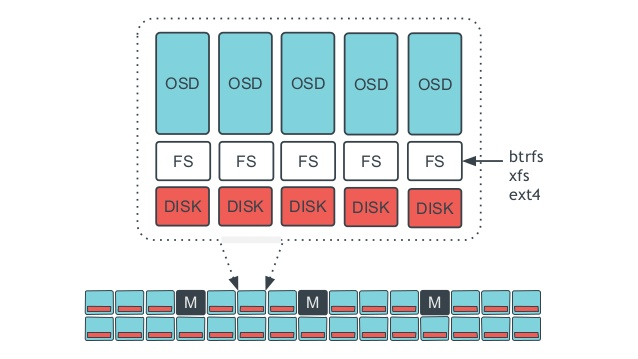
\includegraphics[width=0.8\linewidth]{cluster.jpg}
    \end{figure}
\end{frame}

\begin{frame}{Monitors}
    \begin{itemize}
        \item \textbf{Maintain the cluster map}
            \begin{itemize}
                \item MON map
                \item OSD map
                \item MDS map
                \item PG map
                \item CRUSH map
            \end{itemize}
        \item \textbf{Provide consensus for distributed decision making}
            \begin{itemize}
                \item Each MON knows about all the other MONs in the cluster
                \item First establish a quorum of more than half of MONs so an odd number of MONs is needed in the cluster
                \item MONs in a quorum can distribute maps to OSDs and clients. Clients request cluster maps from a MON only when the primary OSD fails
            \end{itemize}
        \item \textbf{Monitors are not in data path} 
    \end{itemize}
\end{frame}


\begin{frame}{Object Storage Node}
    \begin{itemize}
        \item \textbf{Object Storage Device (OSD)}
            \begin{itemize}   
                \item Building block of Ceph Storage Cluster
                \item One hard disk
                \item One Linux File System
                \item One Ceph OSD Daemon
            \end{itemize}
        \item \textbf{File System:}
            \begin{itemize}
                \item File system must be btrfs, xfs or ext4
                \item Have the XATTRs enabled
            \end{itemize}
   \end{itemize} 
\end{frame}

\begin{frame}{Ceph OSD Daemon}
    \begin{itemize}
        \item \textbf{Ceph Object Storage Device Daemon}
            \begin{itemize}
                \item Serve stored objects to clients
            \end{itemize}
        \item \textbf{OSD is primary for some objects}
            \begin{itemize}
                \item Responsible for replication
                \item Responsible for coherency
                \item Responsible for re-balancing
                \item Responsible for recovery
            \end{itemize}
        \item \textbf{OSD is secondary for some objects}
            \begin{itemize}
                \item Under the control of the primary
                \item Capable of becoming primary
            \end{itemize}
        \item \textbf{Supports extended objects classes}
            \begin{itemize}
                \item Atomic transactions
                \item Synchronization and notifications
                %\item Send computation to the data
            \end{itemize}
    \end{itemize}
\end{frame}

%\begin{frame}{xfs, btrfs, or ext4?}
%    
%\end{frame}

%\begin{frame}{Ceph Journal}
%   
%\end{frame}

\begin{frame}[t]{Ceph Stack}
    \begin{figure}[htpb]
        \centering
        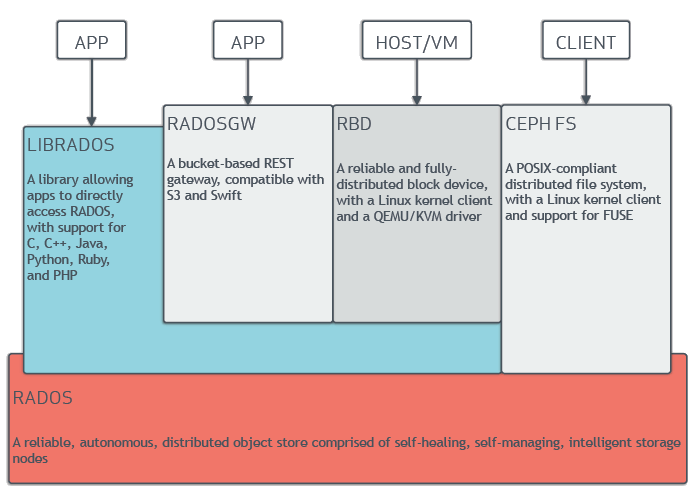
\includegraphics[width=0.75\linewidth]{stack.png}
        \caption{Ceph Stack}
        \label{fig:stack}
    \end{figure}
\end{frame}

\begin{frame}{Communication Methods}
    \begin{tabular}{|c|c|p{0.5\columnwidth}|}
    \hline
        \textbf{Ceph Service}    &   \textbf{Method}  &   \textbf{Description} \\
    \hline
        N/A &   \textit{librados}   &   Library that provides direct access to RADOS for applications \\
    \hline
        Ceph Object Gateway &   \textit{radosgw}    &   RESTful APIs for S3 and Swift compatibility \\
    \hline
        Ceph File System  &   \textit{libcephfs}  &   Library that provides access to Ceph Cluster via a POSIX-like interface \\
    \hline
        Ceph Block Device & \textit{librbd} &   Python module, provides file-like access to RBD images \\
    \hline
    \end{tabular}
\end{frame}

\begin{frame}{RADOSGW}
    \begin{figure}[htpb]
        \centering
        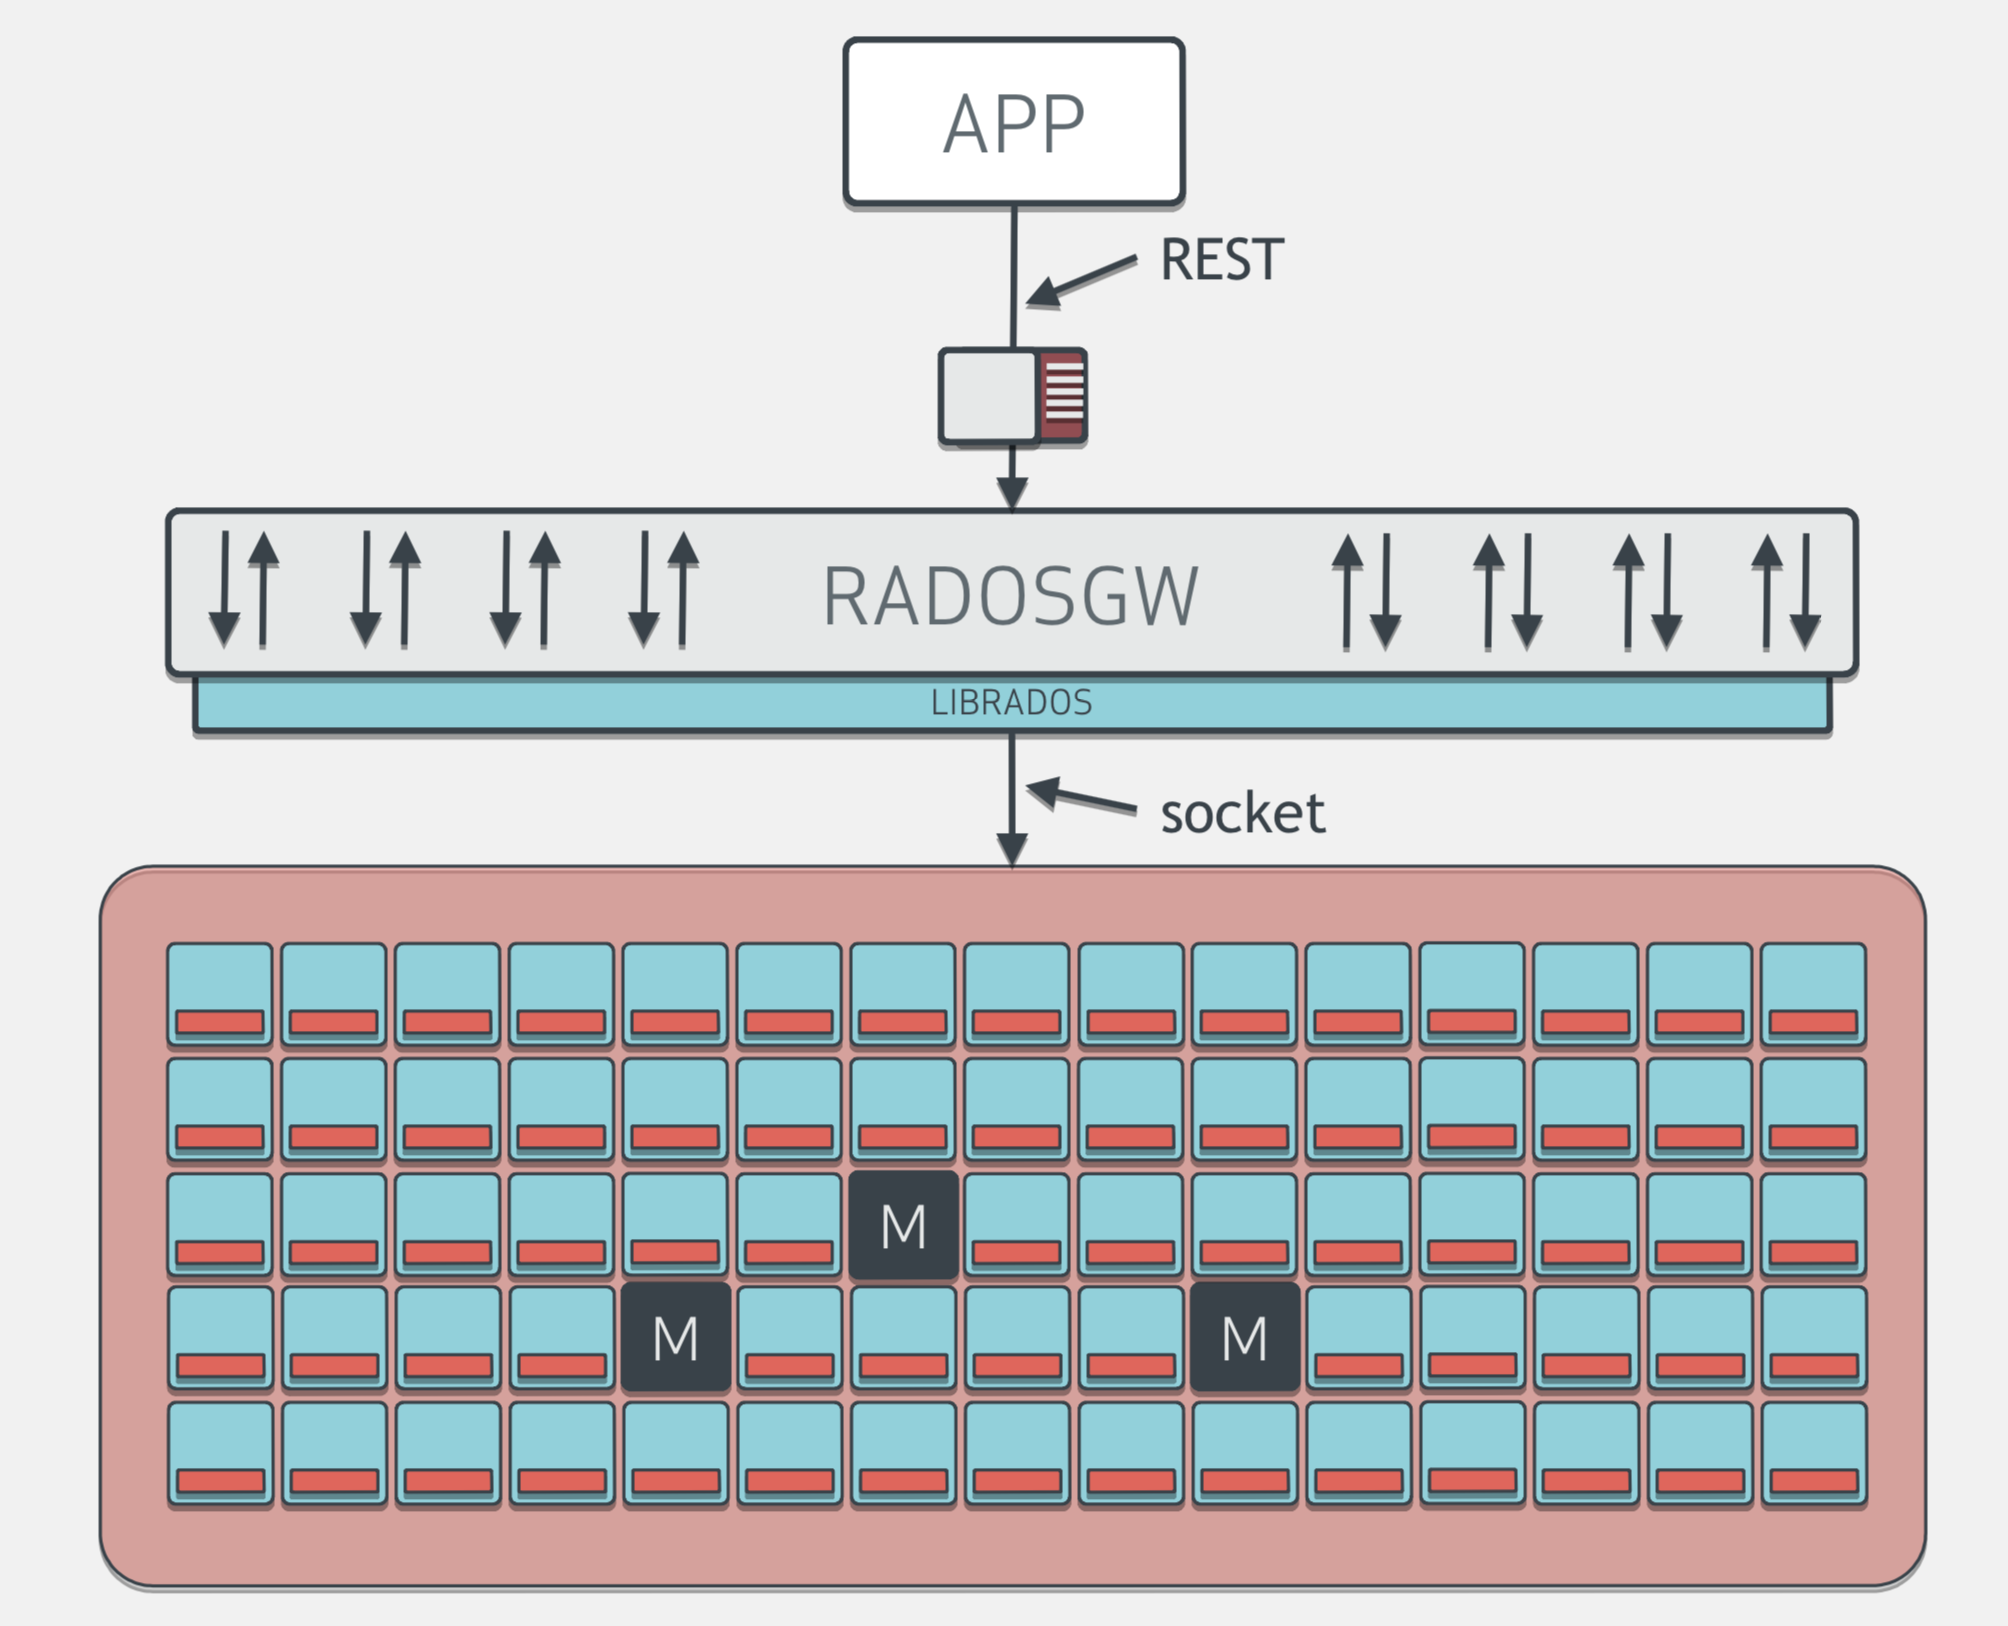
\includegraphics[width=0.7\linewidth]{rgw.png}
    \end{figure}
\end{frame}

\begin{frame}{RBD}
    \begin{figure}[htpb]
        \centering
        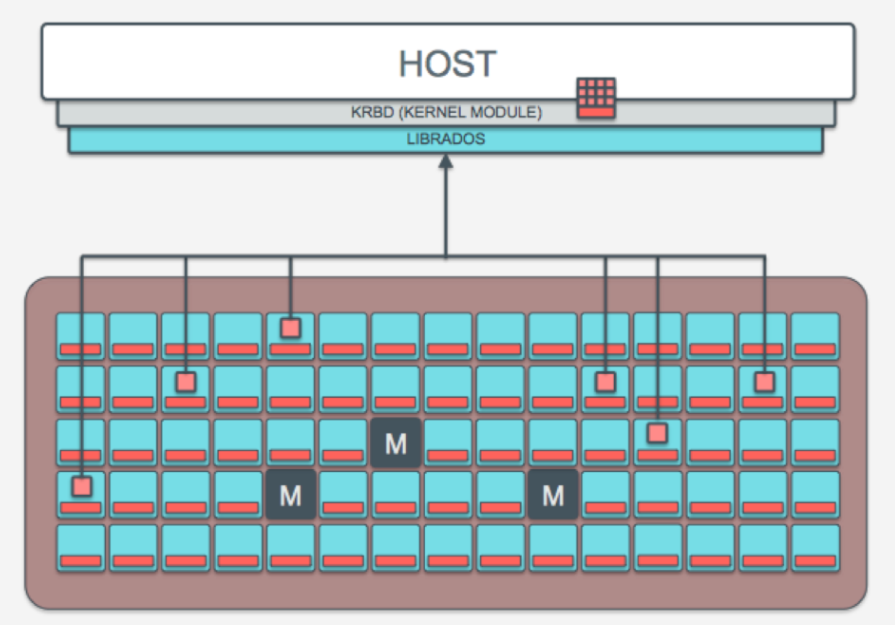
\includegraphics[width=0.8\linewidth]{rbd-native.png}
    \end{figure}
\end{frame}

\begin{frame}{Metadata Server(MDS)}
    \begin{itemize}
        \item \textbf{Manages metadata for a POSIX-compliant shared file system}
            \begin{itemize}
                \item Directory Hierarchy
                \item File Metadata(owner, timestamps, mode, etc)
                \item Stores metadata in Rados
                \item Does not access file content
                \item Only required for shared file system
            \end{itemize}
        \item \textbf{The Ceph Metadata Server daemon}
            \begin{itemize}
                \item Provides the POSIX information needed by file systems that enables CephFS to interact with the Ceph Object Store
                \item It remembers where data lives within a tree
                \item Client accessing CephFS data first make a request to an MDS, which provides what they need to get files from the right OSDs
            \end{itemize}
        \item If you aren't running CephFS, MDS daemons do not need to be deployed. 

    \end{itemize}
\end{frame}

\begin{frame}{CephFS}
    \begin{figure}[htpb]
        \centering
        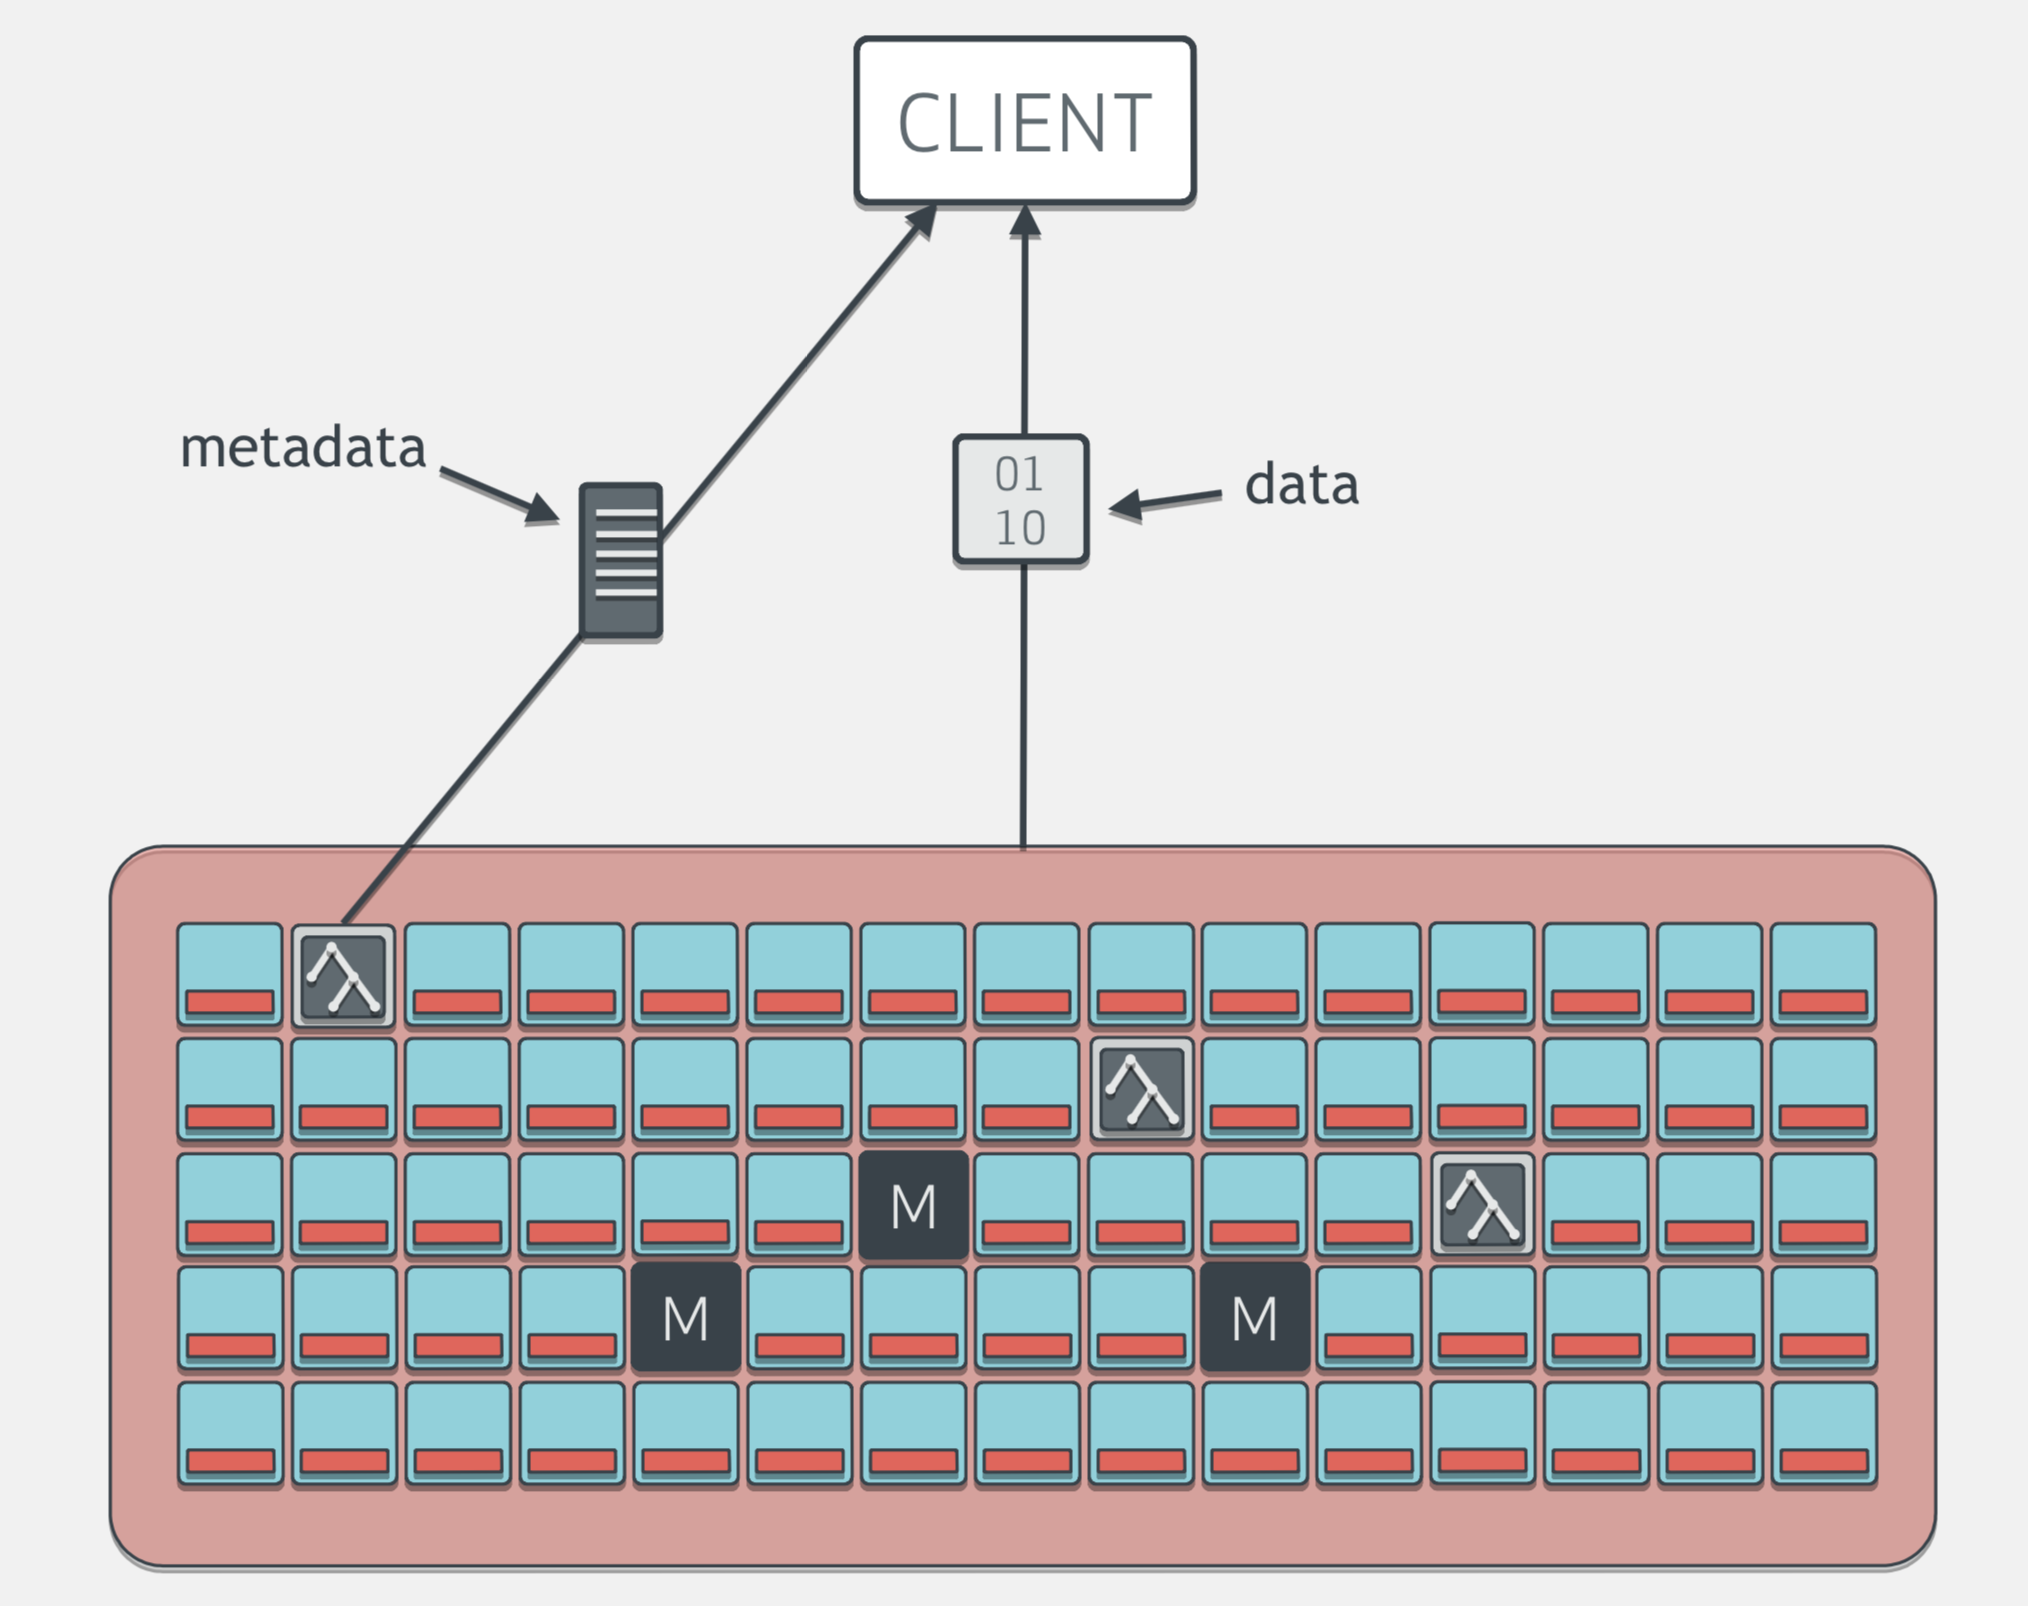
\includegraphics[width=0.7\linewidth]{cephfs.png}
    \end{figure}
\end{frame}

\begin{frame}[fragile]{Ceph Cluster}
\begin{lstlisting}[language=python]
ubuntu@ip-172-31-58-195:~# ceph -s
  cluster:
    id:     ccb00027-ca55-48cc-bf5a-b6cbf79c9b99
    health: HEALTH_OK

  services:
    mon: 3 daemons, quorum ip-172-31-56-105,ip-172-31-57-232,ip-172-31-58-195
    mgr: ip-172-31-56-105(active), standbys: ip-172-31-57-232, ip-172-31-58-195
    mds: cephfs-1/1/1 up  {0=ip-172-31-58-195=up:active}, 2 up:standby
    osd: 4 osds: 3 up, 3 in
    rgw: 1 daemon active

  data:
    pools:   8 pools, 184 pgs
    objects: 268  objects, 37 MiB
    usage:   3.1 GiB used, 87 GiB / 90 GiB avail
    pgs:     184 active+clean    
\end{lstlisting}
\end{frame}

\begin{frame}{Pools and Placement Groups}
    \begin{figure}[htpb]
        \centering
        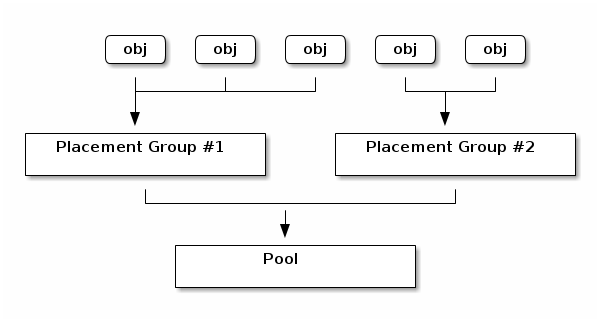
\includegraphics[width=0.8\linewidth]{placement-groups.png}
    \end{figure}
\end{frame}

\begin{frame}{Pools}
    \begin{itemize}
        \item \textbf{What are pools?}
            \begin{itemize}
                \item Pools are logical partitions for storing object data
            \end{itemize}
        \item \textbf{Pools have the following attributes:}
            \begin{itemize}
                \item Set ownership/access
                \item Set number of object replicas
                \item Set number of placement groups
                \item Set the CRUSH rule set to use
            \end{itemize}
        \item \textbf{The PGs within a pool are dynamically mapped to OSDs}
    \end{itemize}
\end{frame}

\begin{frame}[fragile]{Pools}
\begin{lstlisting}[language=python]
ubuntu@ip-172-31-58-195:~# ceph osd lspools
1 .rgw.root
2 default.rgw.control
3 default.rgw.meta
4 default.rgw.log
5 cephfs_data
6 cephfs_metadata
7 rbd
8 default.rgw.buckets.index
ubuntu@ip-172-31-58-195:~# rados df
POOL_NAME                    USED OBJECTS CLONES COPIES ... RD_OPS      RD WR_OPS     WR
cephfs_data                  28 B       2      0      6 ...      2   1 KiB      2  2 KiB
cephfs_metadata            13 KiB      22      0     66 ...      5   5 KiB     91 46 KiB
...
rbd                        37 MiB      19      0     57 ...   2522 5.3 MiB   1313 81 MiB

total_objects    268
total_used       3.1 GiB
total_avail      87 GiB
total_space      90 GiB 
ubuntu@ip-172-31-58-195:~#  ceph osd pool create {pool-name} {pg-num} [{pgp-num}]
\end{lstlisting}
\end{frame}

\begin{frame}{Placement Groups (PGs)}
    \begin{itemize}
        \item \textbf{What is a PG?}
            \begin{itemize}
                \item A PG is a logical collection of objects
                \item Objects within the PG are replicated by the same set of OSDs
            \end{itemize}
        \item \textbf{How to choose the PG?}
            \begin{itemize}
                \item An object's PG is determined by hashing the object name against the number of PGs in the pool
                \item A PG's location is determined by CRUSH according to desired protection and placement strategies
            \end{itemize}
    \end{itemize}
\end{frame}

\begin{frame}{Placement Groups (PGs)}
    \begin{figure}[htpb]
        \centering
        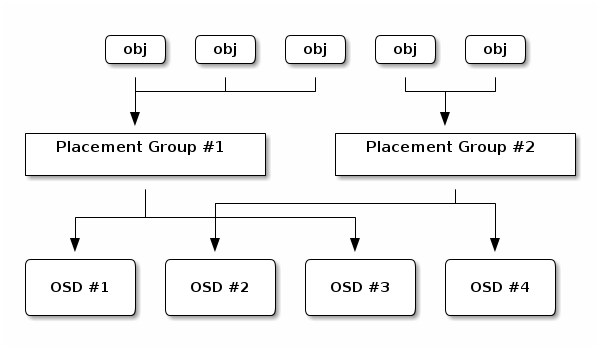
\includegraphics[width=0.8\linewidth]{pg2osd.png}
    \end{figure}
\end{frame}

\begin{frame}{Placement Groups (PGs)}
    \begin{itemize}
        \item \textbf{Without them}
            \begin{itemize}
                \item Track placement and metadata on per-object basis
                \item Not realistic nor scalable with a million++ objects
            \end{itemize}
        \item \textbf{Extra Benefits}
            \begin{itemize}
                \item Reduce the number of processes
                \item Reduce amount of per object metadata Ceph must track
            \end{itemize}
        \item \textbf{Handling the cluster life cycle}
            \begin{itemize}
                \item The total number of PGs must be adjusted when growing the cluster
                \item As devices leave or join the Ceph cluster, most PGs remain where they are
                \item Approximately 50-200 PGs per OSD is recommended -> to balance out memory and CPU requirements and per-OSD load
            \end{itemize}
    \end{itemize}
\end{frame}

\begin{frame}{From Object to OSD}
    \begin{figure}[htpb]
        \centering
        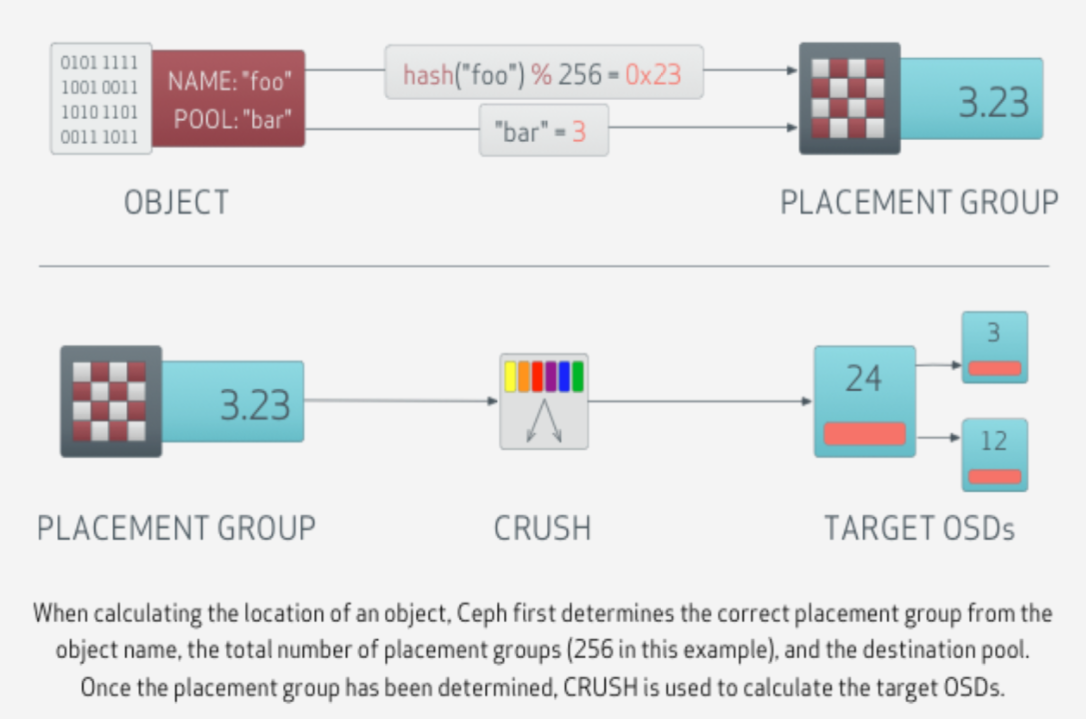
\includegraphics[width=0.8\linewidth]{object2osd.png}
    \end{figure}
\end{frame}

\section{Data Placement}

\subsection{Object Address}

\begin{frame}{Object Addressing}
    \begin{figure}[htpb]
        \centering
        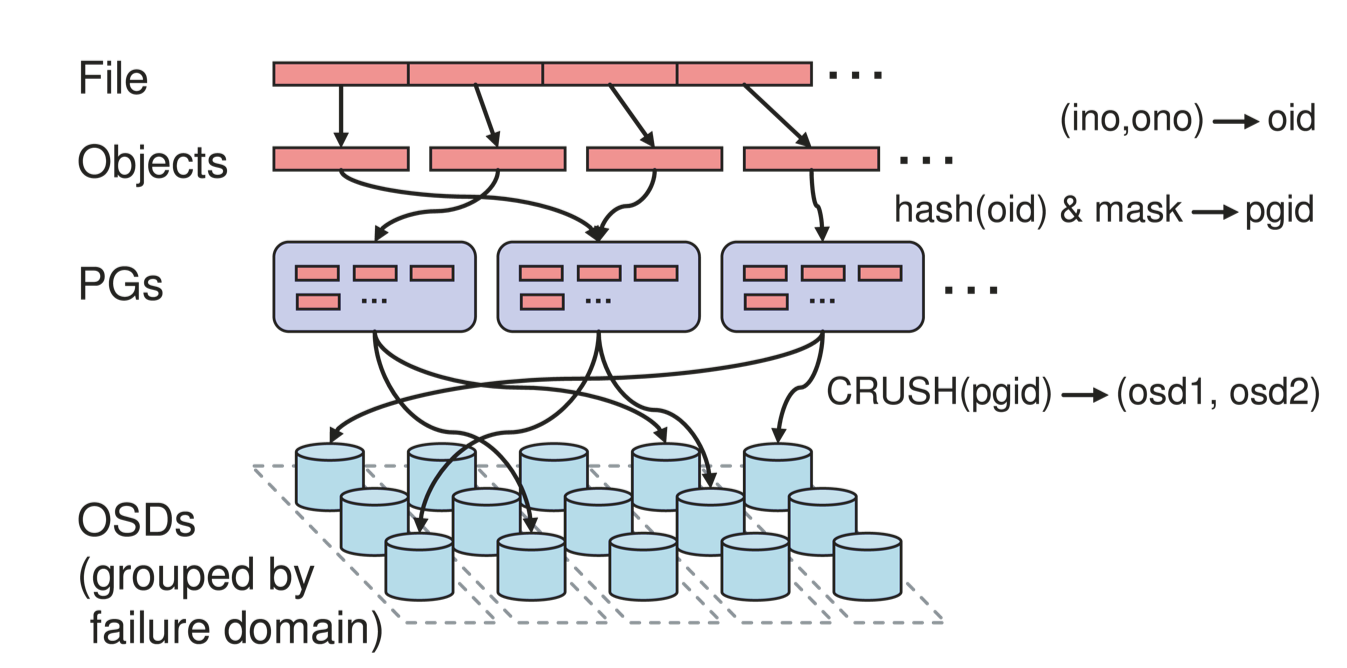
\includegraphics[width=0.8\linewidth]{data-distribution.png}
    \end{figure}
\end{frame}

\begin{frame}{寻址流程}
    \begin{itemize}
        \item \textbf{File -> Object}
            \begin{itemize}
                \item 将用户要操作的File,映射成RADOS能够处理的Object
                \item 本质上是按照Object的最大Size对File进行切分
                \item 切分可以使大小不限的File变成最大Size一致、可以被RADOS高效管理的Object
                \item 切分同时也可以让对单一File实施的串行处理变成对多个Object实施的并行化处理
            \end{itemize}
        \item \textbf{Object -> PG}
            \begin{itemize}
                \item 将每个Object独立的映射到一个PG中去
                \item 固定的Hash算法
            \end{itemize}
        \item \textbf{PG -> OSD}
            \begin{itemize}
                \item 将作为Object的逻辑组织单元的PG映射到数据的实际存储单元OSD
                \item 采用CRUSH算法
            \end{itemize}
    \end{itemize}
\end{frame}

\begin{frame}{CRUSH Function}
    \begin{figure}[htpb]
        \centering
        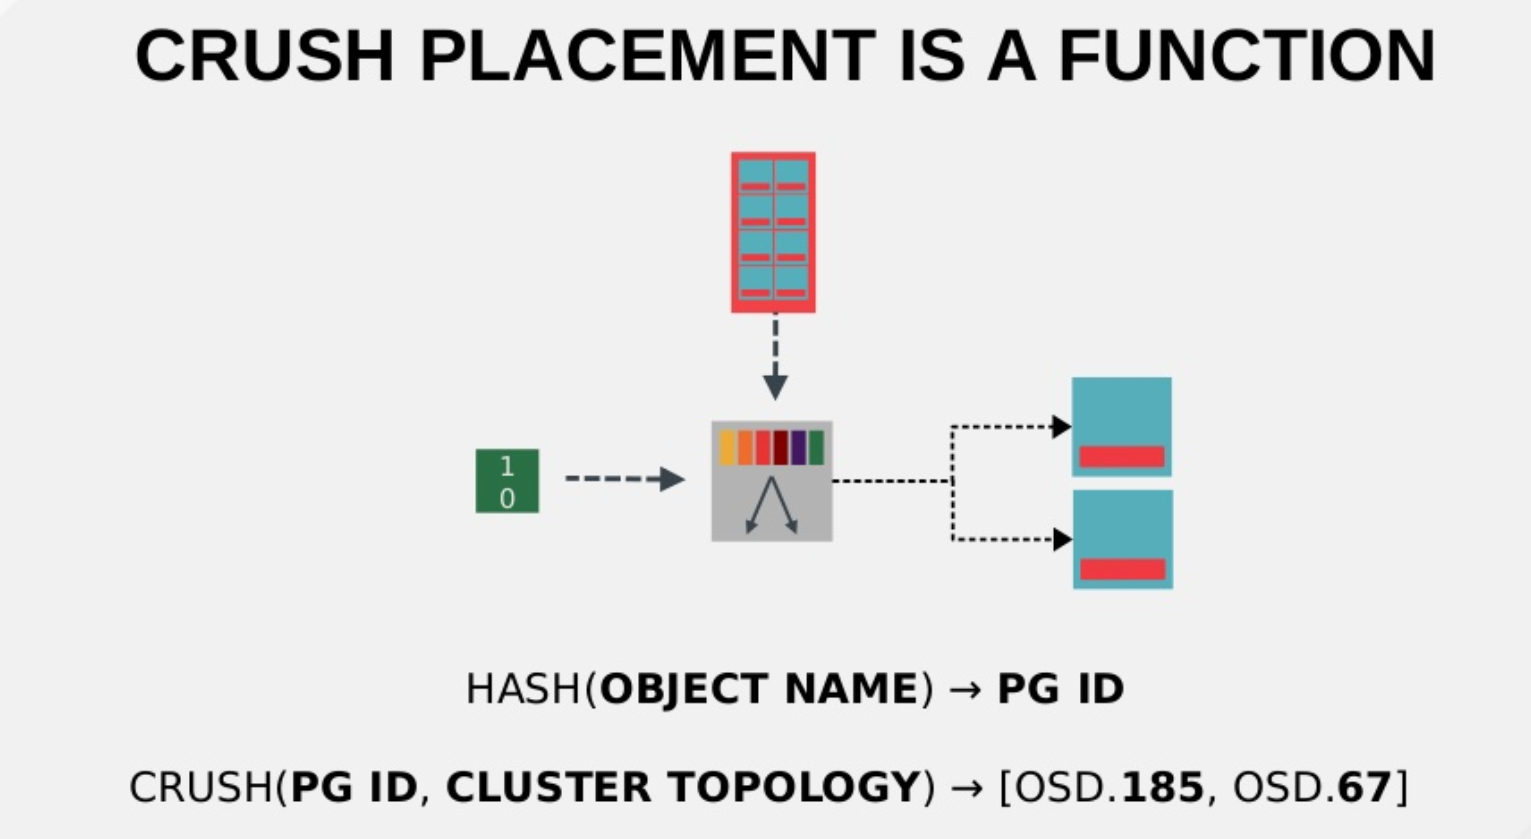
\includegraphics[width=0.9\linewidth]{crush-function.png}
    \end{figure}
\end{frame}

\begin{frame}{CRUSH}
    \begin{itemize}
        \item CRUSH(x) -> ($osd_{n1}, osd_{n2}, osd_{n3}$)
            \begin{itemize}
                \item Inputs
                    \begin{itemize}
                        \item x is the placement group
                        \item hierarchical cluster map
                        \item placement rules
                    \end{itemize}
                \item Outputs: a list of OSDs
            \end{itemize}
        \item Advantages
            \begin{itemize}
                \item Anyone can calculate object location
                \item Cluster map infrequently updated
            \end{itemize}
    \end{itemize}
\end{frame}

\begin{frame}{CRUSH}
    \begin{figure}[htpb]
        \centering
        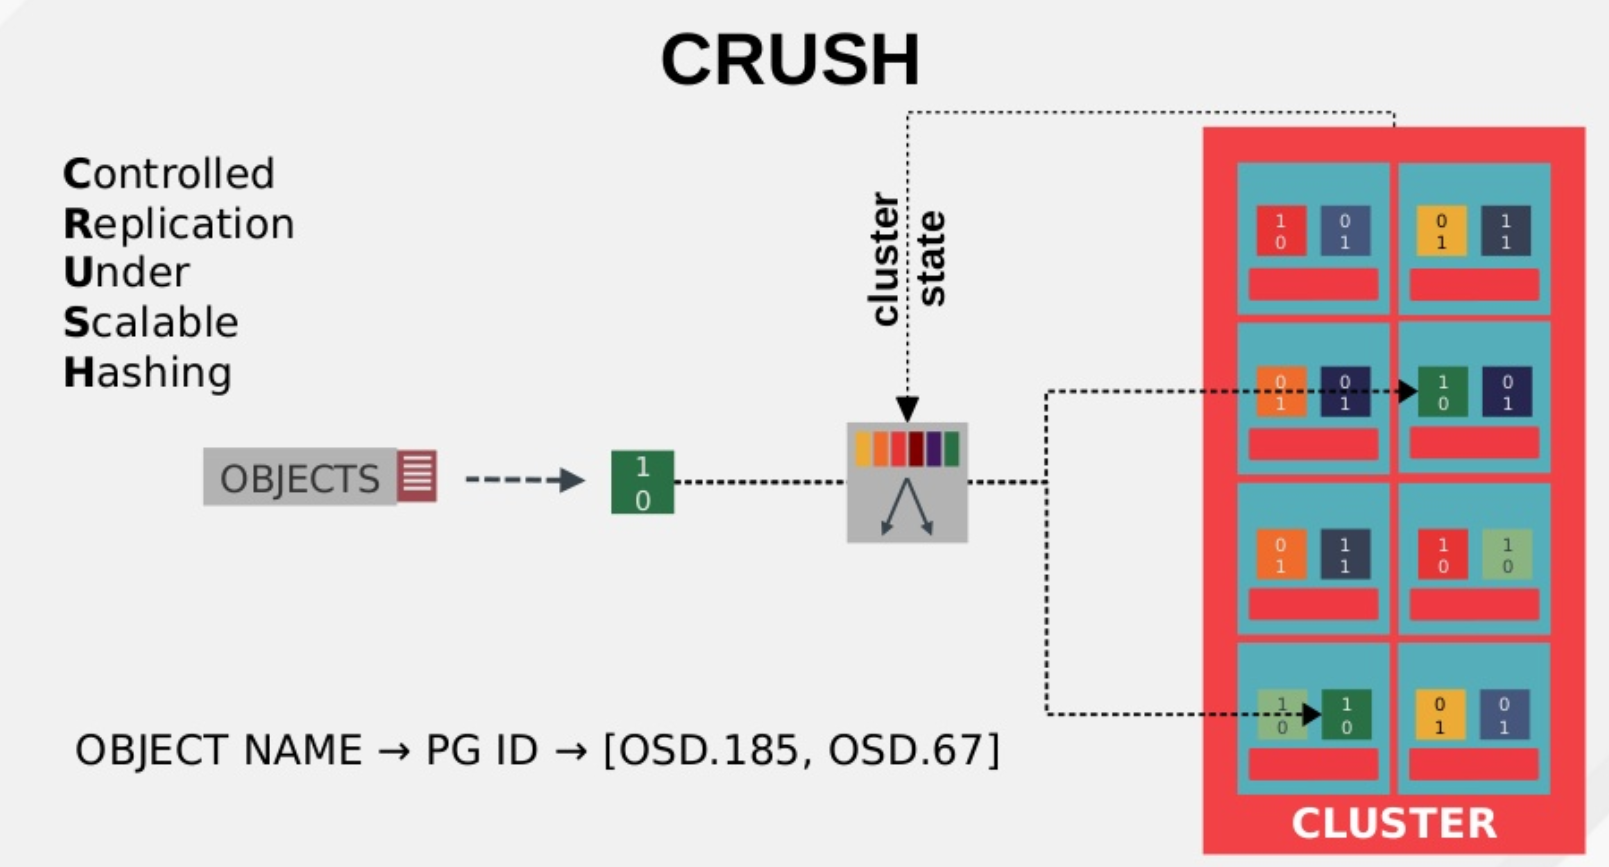
\includegraphics[width=0.9\linewidth]{crush.png}
    \end{figure}
\end{frame}

\begin{frame}{CRUSH}
    CRUSH(Controlled Replication Under Scalable Hashing)
    \begin{itemize}
        \item \textbf{Ceph's data distribution mechanism}
        \item \textbf{Pseudo-random placement algorithm}
            \begin{itemize}
                \item Deterministic function of inputs
                \item Clients can compute data location
            \end{itemize}
        \item \textbf{Rule-based configuration}
            \begin{itemize}
                \item Desired/required replica count
                \item Affinity/distribution rules
                \item Infrastructure topology
                \item Weighting
            \end{itemize}
        \item \textbf{Excellent data distribution}
            \begin{itemize}
                \item De-clustered placement
                \item Excellent data-re-distribution
                %\item Migration proportional to change
            \end{itemize}
    \end{itemize}
\end{frame}

\begin{frame}{Key CRUSH Properties}
    \begin{itemize}
        \item \textbf{No Storage} - Only need to know the cluster topology
        \item \textbf{Fast} - microseconds, even for very large clusters
        \item \textbf{Stable} - very little data movement when topology changes
        \item \textbf{Reliable} - placement is constrained by \textbf{\textit{failure domains}}
        \item \textbf{Flexible} - replication, erasure codes, complex placement schemes
    \end{itemize}
\end{frame}

\subsection{Cluster Map}

%\begin{frame}{CRUSH Map Hierarchy}
%    \begin{itemize}
%        \item \textbf{Device list: List of OSDs}
%        \item \textbf{Buckets: Hierarchical aggregation of storage locations}
%            \begin{itemize}
%                \item Buckets have an assigned weight
%                \item Buckets have a type
%                    \begin{itemize}
%                        \item root
%                        \item datacenter
%                        \item rack
%                        \item host
%                        \item osd
%                    \end{itemize}
%            \end{itemize}
%        \item \textbf{Rules: define data placement for pools}
%    \end{itemize}
%\end{frame}
%
%\begin{frame}{CRUSH Map Hierarchy}
%    The CRUSH Map contains
%    \begin{itemize}
%        \item A list of OSDs
%        \item A list of the rules to tell CRUSH how data is to be replicated
%        \item A default CRUSH is created where you create the cluster
%    \end{itemize}
%\end{frame}

\begin{frame}{Hierarchical Cluster Map}
    \begin{itemize}
        \item \textbf{The cluster map is composed of \textit{device} and \textit{bucket}}
        \begin{itemize}
            \item \textbf{device}: basic storage device, OSD
            \item \textbf{bucket}: container, and contain any number of devices or other buckets
            \item \textbf{item}: member of bucket, can be device or lower level bucket
            \item both device and bucket have numerical identifiers and weight values associated with them
        \end{itemize}
        \item bucket type:
            \begin{itemize}
                \item root, region, datacenter, room, row, rack, host
                \item you can define your own bucket type and hierarchy relation
            \end{itemize}
    \end{itemize}
\end{frame}

\begin{frame}[fragile]{Hierarchical Cluster Map}
    \begin{columns}
        \begin{column}{0.35\textwidth}
\begin{lstlisting}[language=python]
# devices
device 0 osd.0 class hdd
device 1 osd.1 class hdd
device 2 osd.2 class hdd
device 3 osd.3 class hdd
\end{lstlisting}

\begin{lstlisting}[language=python]
# buckets
host node1 {
    id -2
    id -3 class hdd
    # weight 1.000
    alg straw2
    hash 0    # rjenkins1
    item osd.0 weight 1.000
}
\end{lstlisting}
\begin{lstlisting}[language=python]
host node2 {
    id -5
    id -6 class hdd
    # weight 1.000
    alg straw2
    hash 0    # rjenkins1
    item osd.1 weight 1.000
}
\end{lstlisting}
        \end{column}
        \begin{column}{0.55\textwidth}
            
\begin{lstlisting}[language=python]
host node3 {
    id -7
    id -8 class hdd
    # weight 2.000
    alg straw2
    hash 0    # rjenkins1
    item osd.2 weight 1.000
    item osd.3 weight 1.000
}
\end{lstlisting}

\begin{lstlisting}[language=python]
root default {
    id -1   # bucket id, 一般为负数
    # weight 4.000 # sum of item's weight
    alg straw2 # algorithm for random select
    hash 0    # rjenkins1 # hash function type
    item node1 weight 1.000
    item node2 weight 1.000
    item node3 weight 2.000
}
\end{lstlisting}
        \end{column}
    \end{columns}
\end{frame}

\begin{frame}{Cluster Map Example}
    \begin{figure}[htpb]
        \centering
        \includegraphics[width=0.7\linewidth]{crush-cluster-map.png}
    \end{figure}
\end{frame}

\begin{frame}{Failure Domains}
    \begin{itemize}
        \item \textbf{CRUSH generates \textit{n} distinct target devices(OSDs)}
            \begin{itemize}
                \item may be replicas or erasure coding shards
            \end{itemize}
        \item \textbf{Separate replicas across failure domains}
            \begin{itemize}
                \item single failure should only compromise one replica
                \item size of failure domain depends on cluster size
                    \begin{itemize}
                        \item disk
                        \item host(NIC, RAM, PS)
                        \item rack(ToR switch)
                        \item row(distribution switch, ...)
                        \item data center(eletricity...)
                    \end{itemize}
                \item based on types in CRUSH hierarchy
            \end{itemize}
        %\item Sources of failure should be aligned
        %    \begin{itemize}
        %        \item per-rack switch and PDU and physical location
        %    \end{itemize}
    \end{itemize}
\end{frame}

\subsection{Placement Rule}


\begin{frame}[fragile]{CRUSH Rules}
    \begin{columns}
        \begin{column}{0.6\textwidth}
            \begin{itemize}
                \item \textbf{Policy}
                    \begin{itemize}
                        \item where to place replicas
                        \item the failure domain
                    \end{itemize}
                \item \textbf{Trivial program}
                    \begin{itemize}
                        \item short sequence of imperative commands
                        \item flexible, extensible
                        \item not particularly nice for humans
                    \end{itemize}
            \end{itemize} 
        \end{column}
        \begin{column}{0.4\textwidth}
\begin{lstlisting}[language=python]
rule flat {
    ruleset 0   # ruleset id
    type replicated
    min_size 1  # 副本最小数量
    max_size 10 # 副本最大数量
    step take root
    step choose fistn 0 type osd
    step emit
}
\end{lstlisting}
       \end{column}
   \end{columns} 
\end{frame}

\begin{frame}{Basic Operation: Step}
    \begin{itemize}
        \item \textbf{take}: choose a bucket(often root bucket)
        \item \textbf{choose}
            \begin{itemize}
                \item \textbf{choose firstn \{num\} type \{bucket-type\}}
                    \begin{itemize}
                        \item 选择num个bucket-type的item
                    \end{itemize}
                \item \textbf{chooseleaf firstn \{num\} type \{bucket-type\}}
                    \begin{itemize}
                        \item 先选择bucket-type类型的item,再递归选择叶子节点的OSD
                    \end{itemize}
                \item meaning of num parameter
                    \begin{itemize}
                        \item if $num == 0$, choose pool-num-replicas buckets(all available)
                        \item if $num > 0 and < pool-num-replicas$, choose that many buckets
                        \item if $num < 0$, it means $pool-num-replicas - num$
                    \end{itemize}
            \end{itemize}
        \item \textbf{emit} 
    \end{itemize} 
\end{frame}

\begin{frame}[fragile]{RuleSet}
\begin{lstlisting}[language=python]
rule replicated_ruleset {
    ruleset 0       # ruleset id
    type replicated # type replicated or erasure code

    min_size 1
    max_size 10

    step take root
    step choose firstn 1 type row
    step choose firstn 3 type cabinet
    step choose firstn 1 type osd
    step emit
}
\end{lstlisting}
\end{frame}

\begin{frame}{CRUSH Rules}
    \begin{figure}[htpb]
        \centering
        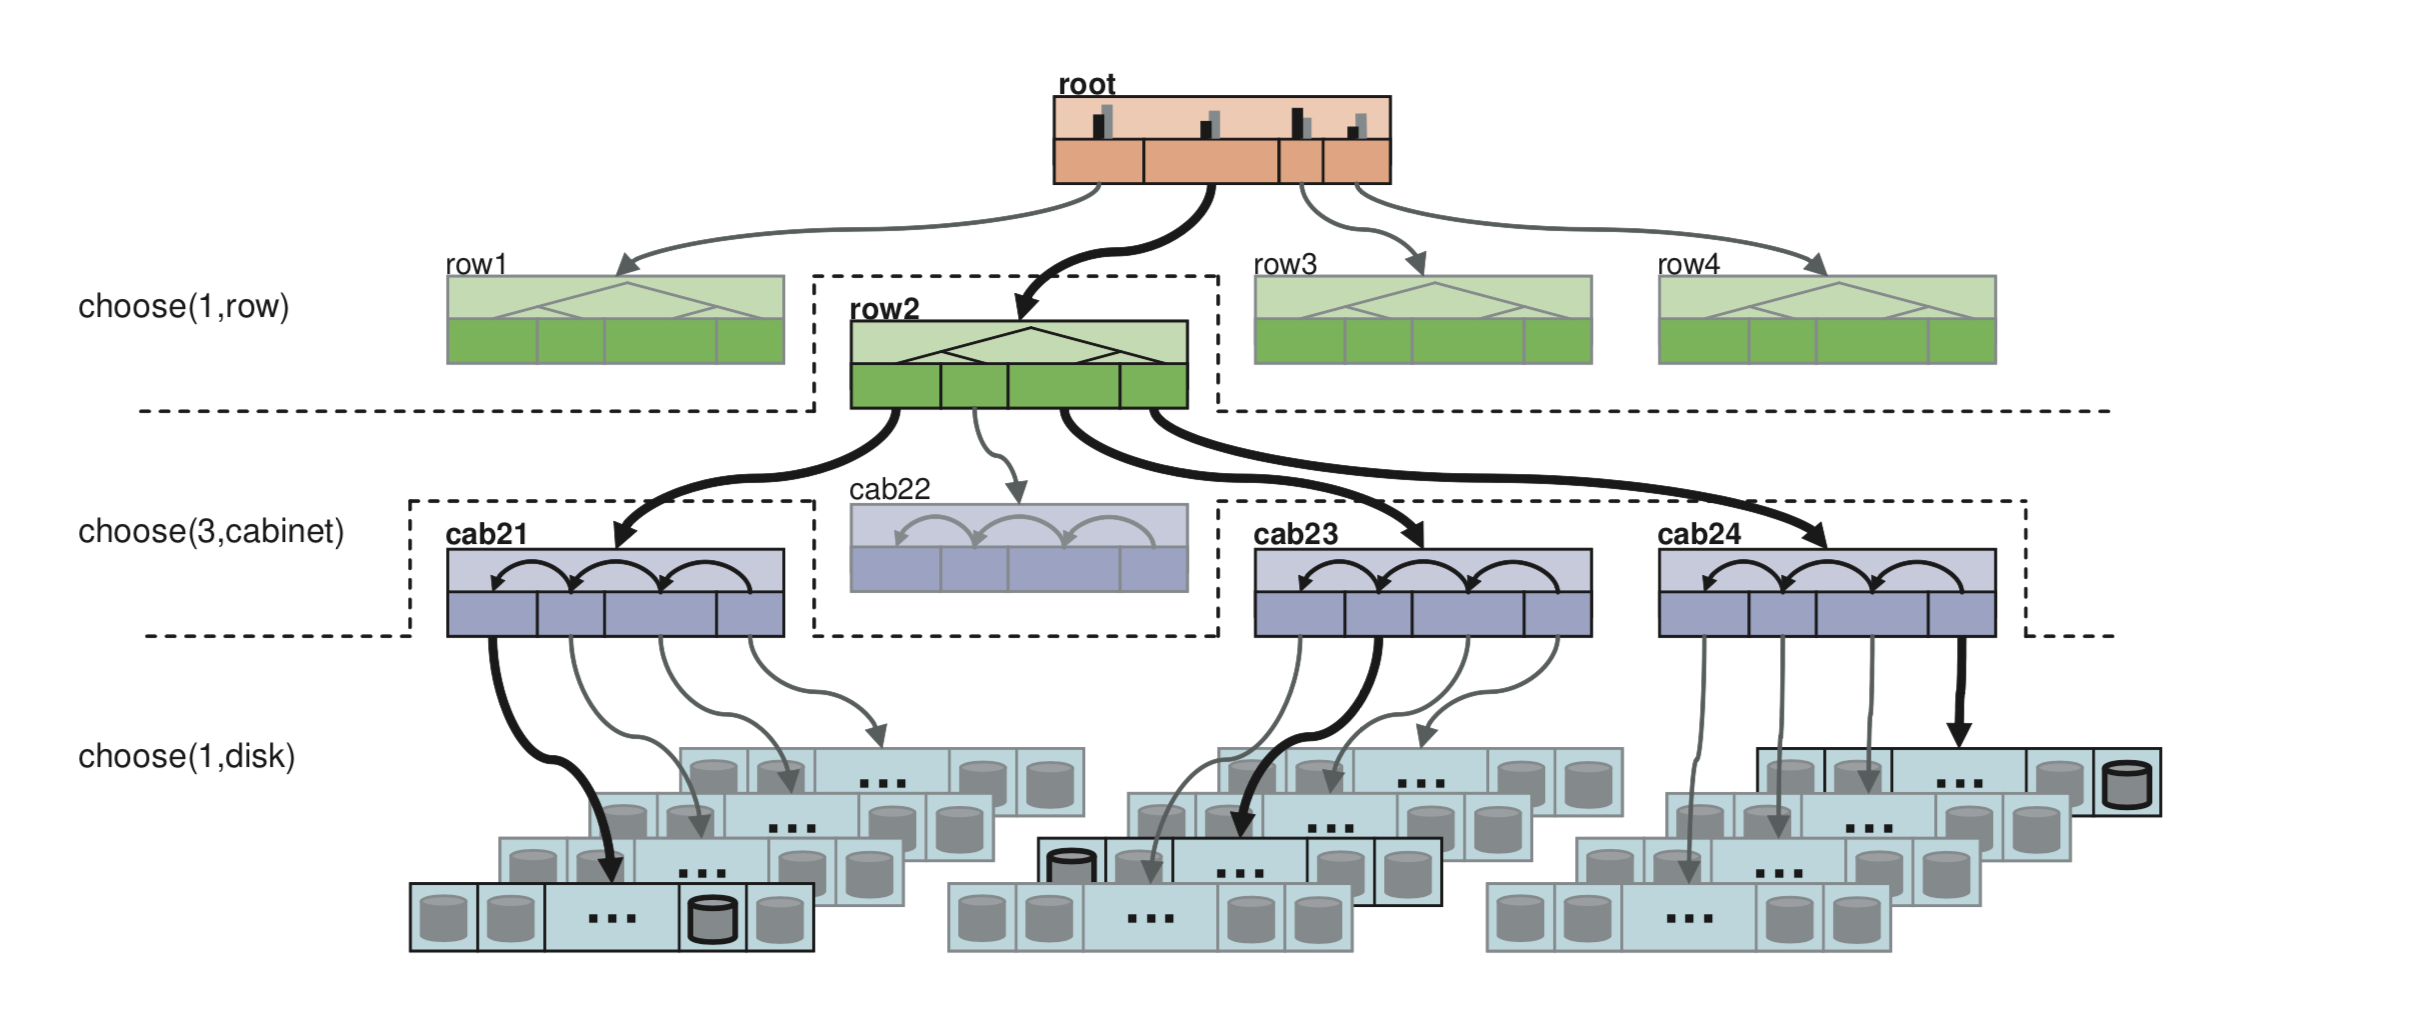
\includegraphics[width=1\linewidth]{crush-ruleset.png}
    \end{figure}
\end{frame}

\begin{frame}[fragile]{RuleSet Example}
\begin{lstlisting}[language=python]
rule ssd-primary {
    ruleset 5       # ruleset id
    type replicated # type replicated or erasure code

    min_size 5
    max_size 10

    step take ssd   # 选择ssd这个root bucket作为输入
    step chooseleaf firstn 1 type host   # 选择一个host,再递归选择叶子节点的osd
    step emit

    step take hdd   # 选择hdd这个root bucket作为输入
    step chooseleaf firstn -1 type host   # 选择总副本数减一个host,再递归选择叶子节点的osd
    step emit
}
\end{lstlisting}
\end{frame}

\begin{frame}{Bucket Algorithms}
    \begin{itemize}
        \item \textbf{Goal of CRUSH algorithm}
            \begin{itemize}
                \item efficiency and scalability of the mapping algorithm
                \item minimum data migration to restore a balanced distribution when the cluster changes due to the addition or removal of devices.
            \end{itemize}
        \item \textbf{CRUSH define 4 kinds of buckets to represent internal nodes in the cluster hierarchy}
            \begin{itemize}
                \item uniform buckets
                \item list buckets
                \item tree buckets
                \item straw buckets
            \end{itemize}
        \item Each bucket type is based on a \textbf{different internal data structure} and utilizes a \textbf{different function c(r, x) for pseudo-randomly choosing nested items} during the replica placement process
        \item Each bucket type represents a different \textbf{tradeoff between computation and reorganization efficiency}
    \end{itemize}
\end{frame}

\begin{frame}{How does it work?}
    \begin{figure}[htpb]
        \centering
        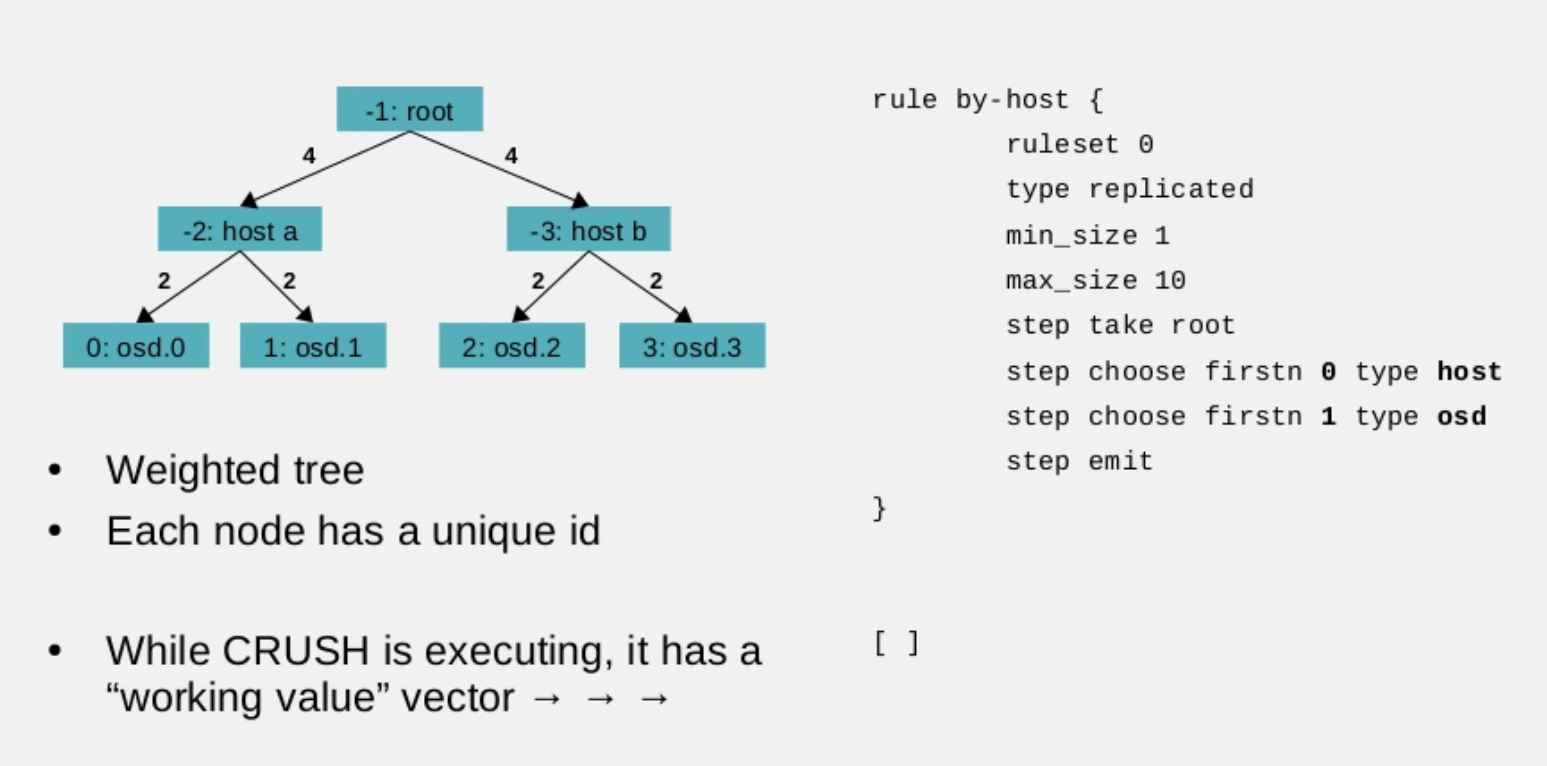
\includegraphics[width=0.8\linewidth]{crush0.png}
    \end{figure}
\end{frame}

\begin{frame}{How does it work?}
    \begin{figure}[htpb]
        \centering
        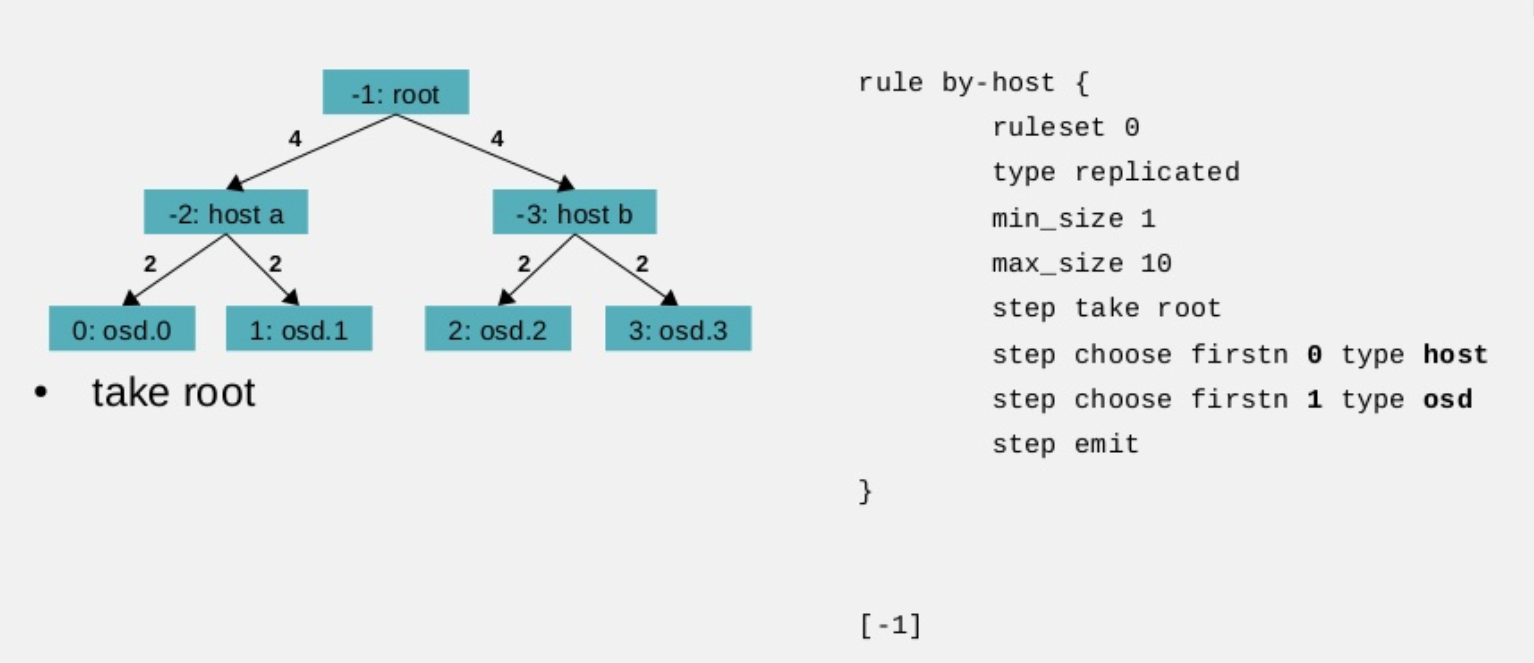
\includegraphics[width=0.8\linewidth]{crush1.png}
    \end{figure}
\end{frame}

\begin{frame}{How does it work?}
    \begin{figure}[htpb]
        \centering
        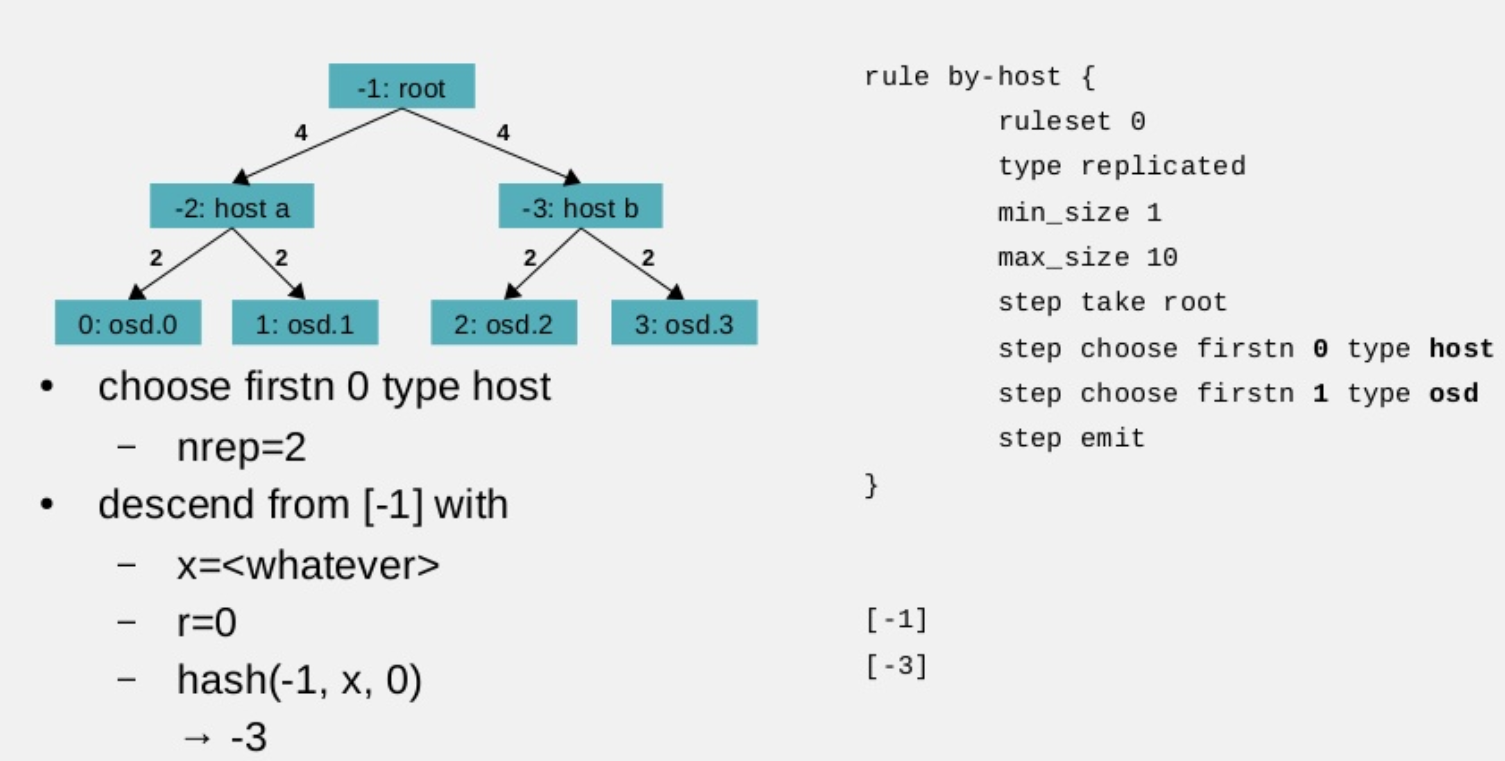
\includegraphics[width=0.8\linewidth]{crush2.png}
    \end{figure}
\end{frame}

\begin{frame}{How does it work?}
    \begin{figure}[htpb]
        \centering
        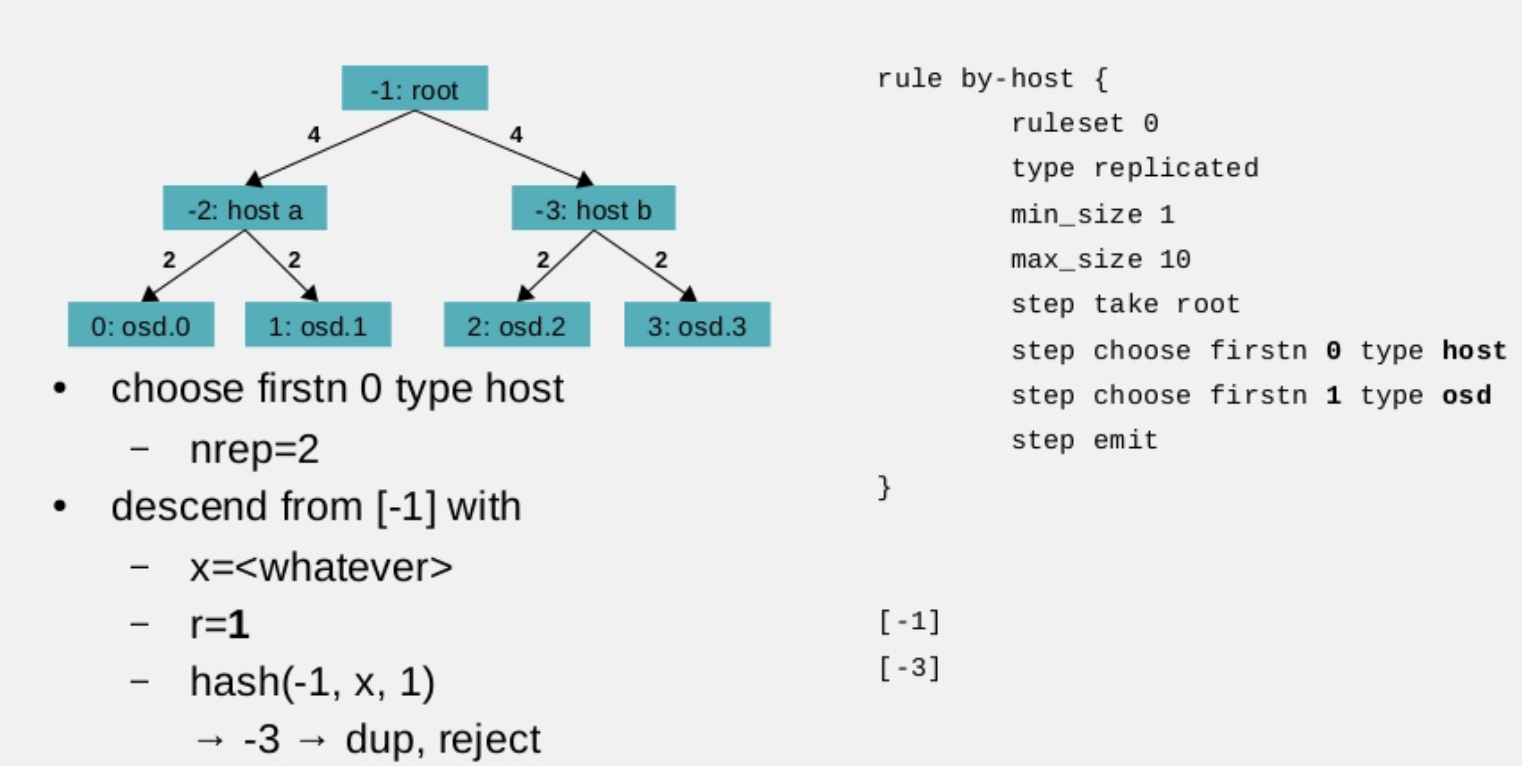
\includegraphics[width=0.8\linewidth]{crush3.png}
    \end{figure}
\end{frame}

\begin{frame}{How does it work?}
    \begin{figure}[htpb]
        \centering
        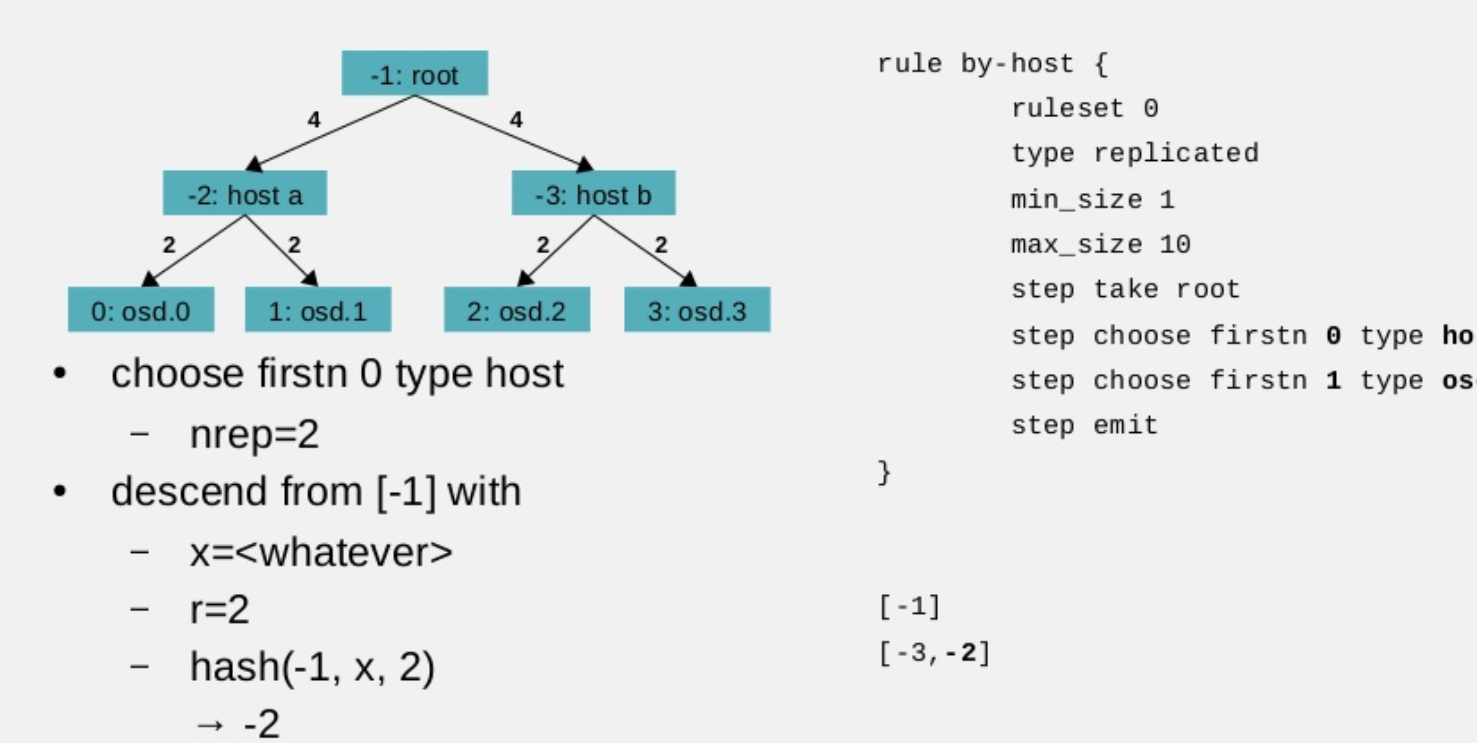
\includegraphics[width=0.8\linewidth]{crush4.png}
    \end{figure}
\end{frame}

\begin{frame}{How does it work?}
    \begin{figure}[htpb]
        \centering
        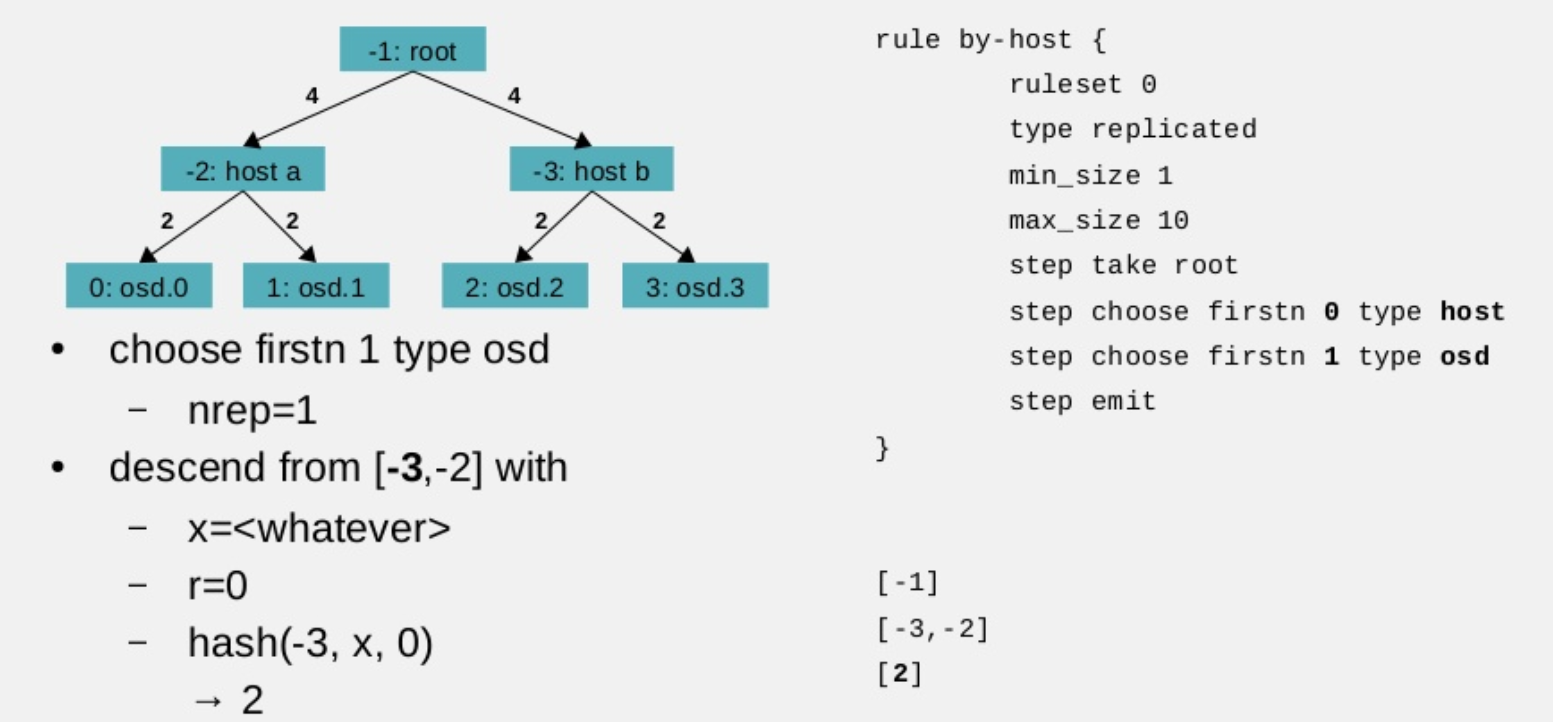
\includegraphics[width=0.8\linewidth]{crush5.png}
    \end{figure}
\end{frame}

\begin{frame}{How does it work?}
    \begin{figure}[htpb]
        \centering
        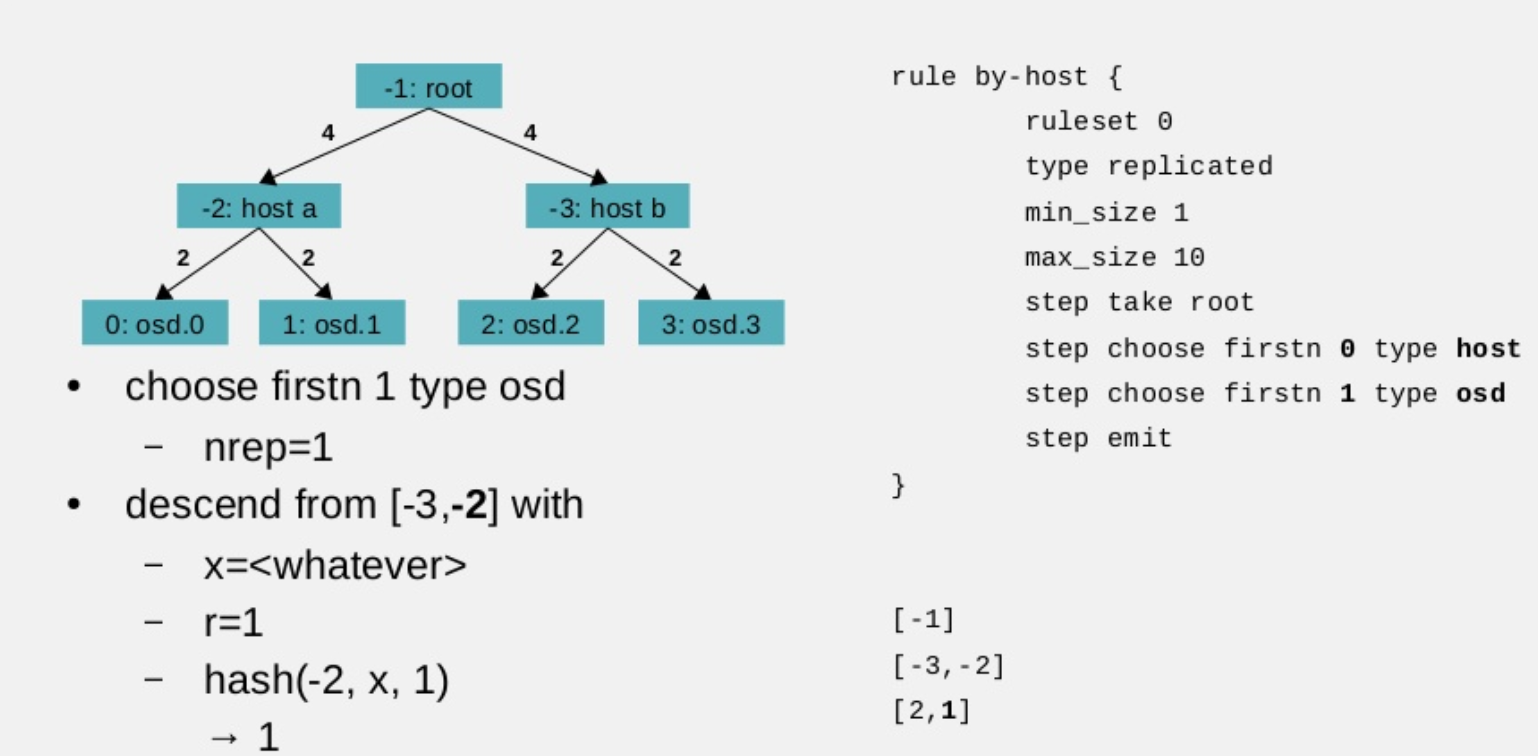
\includegraphics[width=0.8\linewidth]{crush6.png}
    \end{figure}
\end{frame}

\begin{frame}{Bucket Algorithms}
    \begin{itemize}
        \item \textbf{Many algorithms for selecting a child}
            \begin{itemize}
                \item every internal tree node has a type
                \item tradeof between time/computation and rebalancing behavior
                \item can mix types within a tree
            \end{itemize}
        \item \textbf{uniform}
            \begin{itemize}
                \item $hash(nodeid, x, r) \% num_children$
                \item fiexed $O(1)$ time
                \item addint child shuffles everything
            \end{itemize}
        \item \textbf{straw2}
            \begin{itemize}
                \item $hash(nodeid, x, r, child)$ for every child
                \item scale based on child weight
                \item pick the biggest value
                \item $O(n)$ time
            \end{itemize}
        \item \textbf{adding or removing child}
            \begin{itemize}
                \item only moves values to or from that child
                \item still fast enough for small n
            \end{itemize}
    \end{itemize}
\end{frame}

%\begin{frame}{Uniform Buckets}
%    
%\end{frame}

%\begin{frame}{List Buckets}
    
%\end{frame}

%\begin{frame}{Tree Buckets}
%    
%\end{frame}

%\begin{frame}{Straw Buckets}
%    
%\end{frame}


\section{Ceph RADOS}

\begin{frame}{Cluster Aware}
    Where should the object be placed
    \begin{itemize}
        \item \textbf{Traditional}
            \begin{itemize}
                \item Centralized interface provides services to the client through a double dispatch
                \item Huge bottleneck at petabyte-to-exabyte scale.
            \end{itemize}
        \item \textbf{Ceph}
            \begin{itemize}
                \item Ceph OSD and Client are \textit{cluster aware}
                \item Each OSD knows about other OSD in the cluster
                \item OSD can interact directly with other OSD and monitors
                \item Client can interact directly with OSD
            \end{itemize}
    \end{itemize}
\end{frame}

%\begin{frame}{Cluster Aware}
%    \begin{itemize}
%        \item \textbf{OSDs Service Clients Directly}
%        \item \textbf{OSD Membership and Status}
%        \item \textbf{Data Scrubbing}
%        \item \textbf{Replication}
%    \end{itemize}
%\end{frame}

\begin{frame}{Cluster Map}
    Cluster Map indicates the knowledge of the cluster topology.
    \begin{itemize}
        \item \textbf{The Monitor Map}
        \item \textbf{The OSD Map}
        \item \textbf{The PG Map}
        \item \textbf{The CRUSH Map}
        \item \textbf{The MDS Map} 
    \end{itemize}
\end{frame}

\begin{frame}[fragile]{Cluster Map: Monoitor Map}
\begin{lstlisting}[language=python]
ubuntu@ip-172-31-58-195:~# ceph mon dump
dumped monmap epoch 2
epoch 2
fsid ccb00027-ca55-48cc-bf5a-b6cbf79c9b99
last_changed 2018-12-26 18:17:17.540294
created 2018-12-26 18:16:44.542161
0: 172.31.56.105:6789/0 mon.ip-172-31-56-105
1: 172.31.57.232:6789/0 mon.ip-172-31-57-232
2: 172.31.58.195:6789/0 mon.ip-172-31-58-195 
\end{lstlisting}
\end{frame}

\begin{frame}[fragile]{Cluster Map: OSD Map}
\begin{lstlisting}[language=python]
ubuntu@ip-172-31-58-195:~# ceph osd dump
epoch 245
fsid ccb00027-ca55-48cc-bf5a-b6cbf79c9b99
created 2018-12-26 18:17:10.141095
modified 2018-12-29 12:02:43.764006
crush_version 26
...
pool 5 'cephfs_data' replicated size 3 min_size 2 crush_rule 0 object_hash rjenkins pg_num 64 pgp_num 64 last_change 48 flags hashpspool stripe_width 0 application cephfs
pool 6 'cephfs_metadata' replicated size 3 min_size 2 crush_rule 0 object_hash rjenkins pg_num 64 pgp_num 64 last_change 48 flags hashpspool stripe_width 0 application cephfs
max_osd 4
osd.0 up   in  weight 1 up_from 98 up_thru 244 down_at 94 last_clean_interval [90,93) 172.31.56.105:6801/2052 172.31.56.105:6802/2052 172.31.56.105:6803/2052 172.31.56.105:6804/2052 exists,up 2ee23b61-eca4-41e5-a6b0-277bfd6c48a1
...
\end{lstlisting}
\end{frame}

\begin{frame}[fragile]{Cluster Map: CRUSH Map}
\begin{lstlisting}[language=python]
ubuntu@ip-172-31-58-195:~# ceph osd tree
ID CLASS WEIGHT  TYPE NAME                 STATUS REWEIGHT PRI-AFF
-1       0.11597 root default
-3       0.02899     host ip-172-31-56-105
 0   ssd 0.02899         osd.0                 up  1.00000 1.00000
-5       0.02899     host ip-172-31-57-232
 1   ssd 0.02899         osd.1                 up  1.00000 1.00000
-7       0.02899     host ip-172-31-58-195
 2   ssd 0.02899         osd.2                 up  1.00000 1.00000
-9       0.02899     host ip-172-31-61-170
 3   ssd 0.02899         osd.3               down        0 1.00000
\end{lstlisting}
\end{frame}

\begin{frame}{Cluster Map}
    \begin{itemize}
        \item 由若干个monitor共同负责整个Ceph集群中所有的OSD状态的发现与记录,并且共同形成cluster map的master版本,然后扩散到整体OSD以及client
        \item OSD使用cluster map进行数据的维护,client使用cluster进行数据的寻址
        \item monitor并不主动轮询各个OSD的当前状态。正相反,OSD需要向monitor上报状态信息。常见的上报有两种情况
            \begin{itemize}
                \item 新的OSD被加入集群
                \item 某个OSD发现自身或者其他OSD发生异常
            \end{itemize}
        \item 在收到这些上报信息后,monitor将更新cluster map信息并加以扩散
    \end{itemize}
\end{frame}

\begin{frame}{Data Operation Procedure}
    \begin{figure}[htpb]
        \centering
        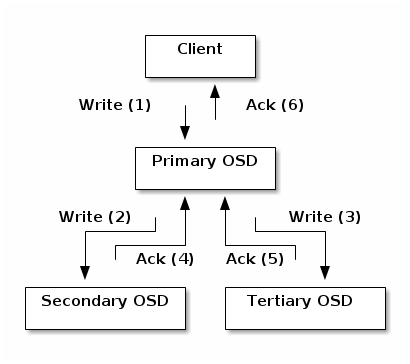
\includegraphics[width=0.6\linewidth]{file-write.png}
    \end{figure}
\end{frame}

\subsection{Map Changes and Data Movement}

\begin{frame}{Peering and Recovery}
    The Ceph Object Store is dynamic
    \begin{itemize}
        \item \textbf{Failure is the norm rather than the exception}
        \item \textbf{The cluster map records cluster state at a point in time}
        \item \textbf{The cluster map contains the OSDs status(up/down, weight, IP)}
            \begin{itemize}
                \item OSDs cooperatively migrate data
                \item They do so to achieve recovery based on CRUSH rules
                \item Any cluster map update potentially triggers data migration
            \end{itemize}
    \end{itemize}
\end{frame}

%\begin{frame}{Failure is the norm}
%    \begin{itemize}
%        \item \textbf{ceph-osd daemon dies}
%            \begin{itemize}
%                \item Peer heartbeats fail; peers inform monitor
%                \item New osdmap published with osd.123 as \textit{down}
%            \end{itemize}
%        \item \textbf{pg maps to fewer replicas}
%            \begin{itemize}
%                \item If osd.123 was primary in a PG, a replica takes over
%                \item PG is \textit{degraded}(N-1 replicas)
%                \item Data redistribution is not triggered
%            \end{itemize}
%        \item \textbf{Monitor marks OSD \textit{out} after 5 minutes}
%            \begin{itemize}
%                \item PG now maps to N OSDs again
%                \item PG re-peers, activates
%                \item Primary backfills to the \textit{new} OSD 
%            \end{itemize}
%    \end{itemize}
%\end{frame}

\begin{frame}{CRUSH}
    \begin{figure}[htpb]
        \centering
        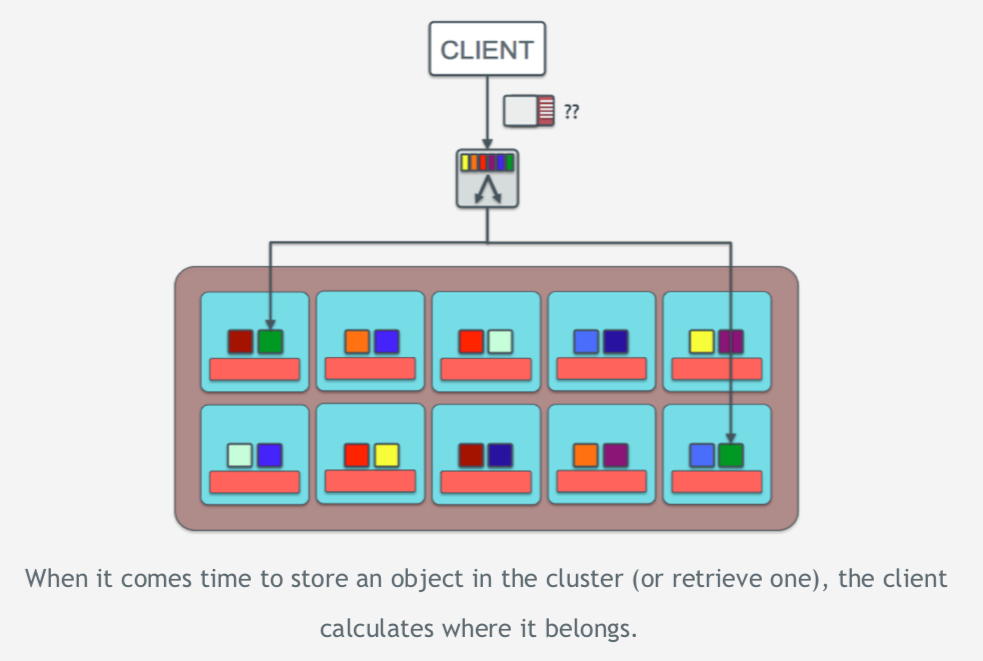
\includegraphics[width=0.8\linewidth]{migration1.png}
    \end{figure}
\end{frame}

\begin{frame}{CRUSH}
    \begin{figure}[htpb]
        \centering
        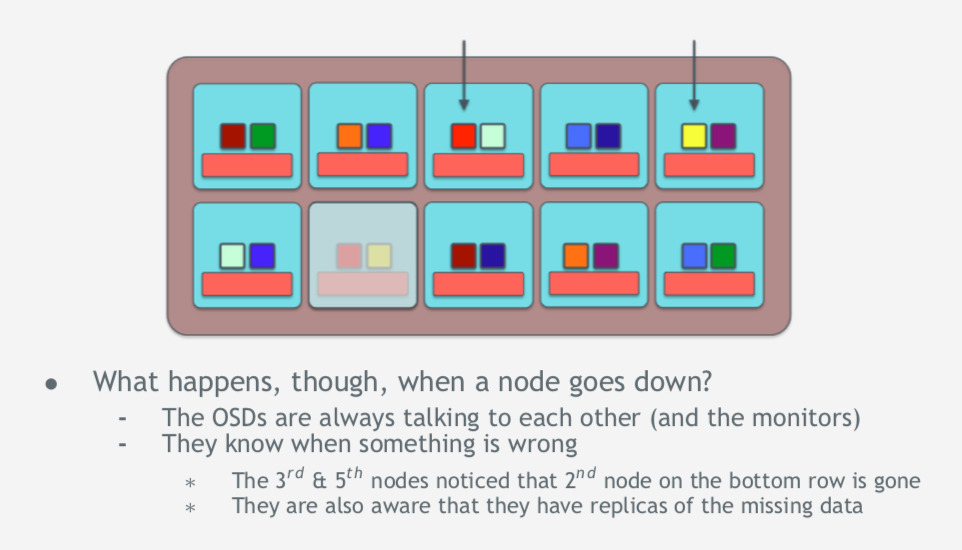
\includegraphics[width=0.8\linewidth]{migration2.png}
    \end{figure}
\end{frame}

\begin{frame}{CRUSH}
    \begin{figure}[htpb]
        \centering
        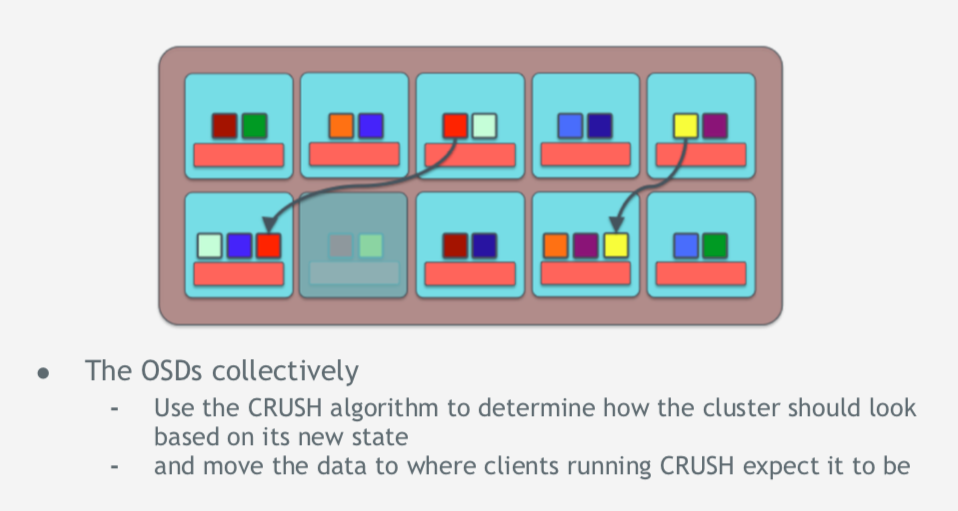
\includegraphics[width=0.8\linewidth]{migration3.png}
    \end{figure}
\end{frame}

\begin{frame}{CRUSH}
    \begin{figure}[htpb]
        \centering
        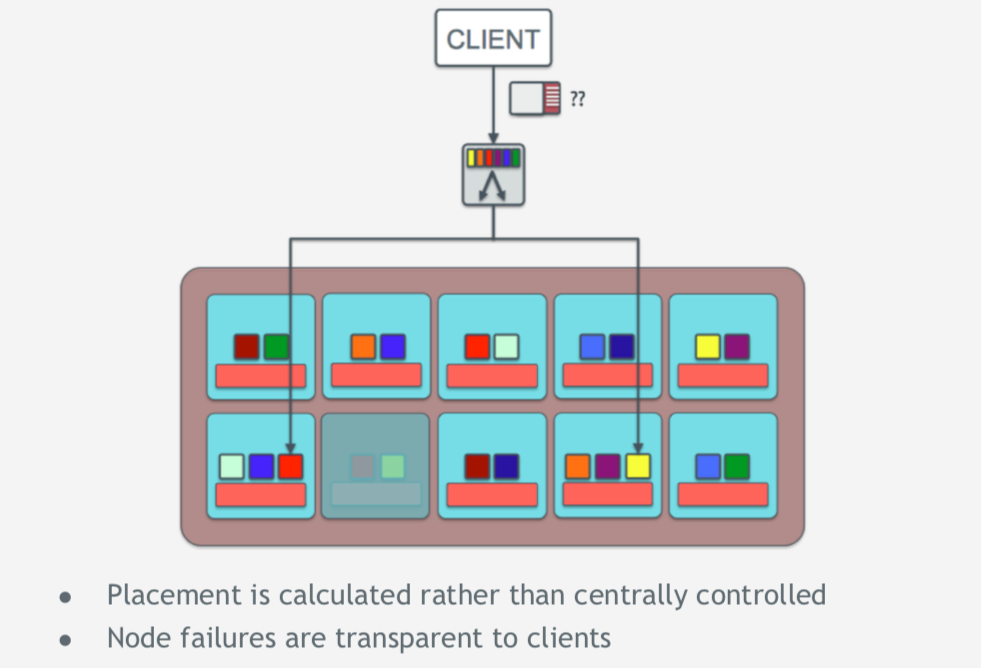
\includegraphics[width=0.8\linewidth]{migration4.png}
    \end{figure}
\end{frame}

\begin{frame}{OSD Fail}
    \begin{figure}[htpb]
        \centering
        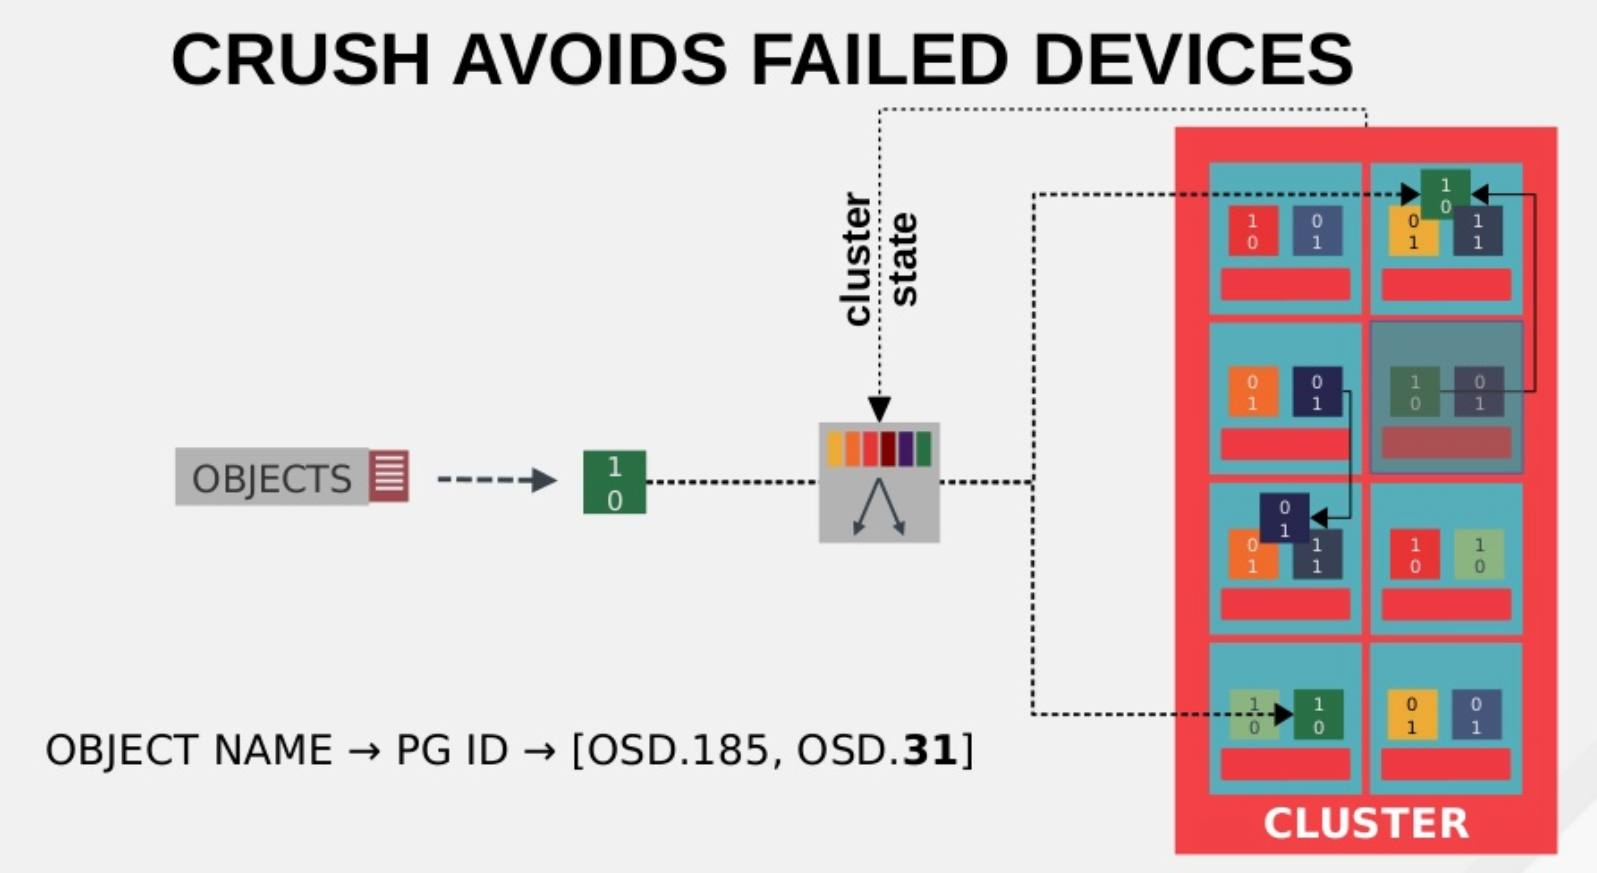
\includegraphics[width=1\linewidth]{crush-failed-device.png}
    \end{figure}
\end{frame}

%\begin{frame}{OSD Expansion}
%    \begin{itemize}
%        \item New rack of OSDs added to CRUSH map
%        \item Many PGs map to new OSDs
%            \begin{itemize}
%                \item Temporarily remap PG to include previous replicas + new OSDs keeps replica count at (or above) target
%                \item Peer and activate
%                \item Background backfill to new OSDs
%                \item Drop re-mapping when completed, activate
%                \item Delete PG data from the old \textit{stray} replica 
%            \end{itemize}
%    \end{itemize}
%\end{frame}
%

\begin{frame}[fragile]{Python S3 Example}
\begin{lstlisting}[language=python]
# creating a connection
conn = boto.connect_s3(aws_access_key_id = access_key,
    aws_secret_access_key = secret_key,
    host = 'objects.dreamhost.com',
    calling_format = boto.s3.connection.OrdinaryCallingFormat())

# listing owned buckets
for bucket in conn.get_all_buckets():
    print "{name}\t{created}".format(name = bucket.name, created = bucket.creation_date)
# mahbuckat1   2011-04-21T18:05:39.000Z
# mahbuckat2   2011-04-21T18:05:48.000Z

# listing a bucket's content
for key in bucket.list():
    print "{name}\t{size}\t{modified}".format(name = key.name, size = key.size, modified = key.last_modified)
# myphoto1.jpg 251262  2011-08-08T21:35:48.000Z
# myphoto2.jpg 262518  2011-08-08T21:38:01.000Z

# creating an object
key = bucket.new_key('hello.txt')
key.set_contents_from_string('Hello World!')

# download an object to a file
key = bucket.get_key('perl_poetry.pdf')
key.get_contents_to_filename('/home/larry/documents/perl_poetry.pdf')

\end{lstlisting}
\end{frame}

\section{Ceph Block Device}

%\begin{frame}{Ceph Block Device - RBD}
%    \begin{itemize}
%        \item Block devices are the most common way to store data
%        \item Allows for storage of virtual disks in the Ceph Object Store
%        \item Allows decoupling of VMs and containers
%        \item High-Performance through data striping across the cluster
%        \item Boot support in QEMU, KVM, and OpenStack(Cinder)
%        \item Mount support in the Linux Kernel
%    \end{itemize}
%\end{frame}

\begin{frame}[fragile]{Create and Mount RBD}
\begin{lstlisting}[language=python]
# create a block device pool
$ ceph osd pool create rbd 128 
$ rbd pool init

# create a block device image(1024MB)
$ rbd create --size 1024 foo
$ rbd list
foo

# map a block device
$ sudo rbd device map rbd/foo --id admin
/dev/rbd0
$ rbd device list
id pool image snap device
0  rbd  foo   -    /dev/rbd0

# format the block device and create a file system
$ sudo mkfs.ext4 -m0 /dev/rbd0
$ sudo mkdir /mnt/rbd
$ sudo mount /dev/rbd/rbd/foo /mnt/rbd

# 查看挂载情况
$ df -h
...
/dev/rbd0            976M  2.6M  958M    1% /mnt/rbd
\end{lstlisting}
\end{frame}

\begin{frame}{RBD: Native}
    \begin{figure}[htpb]
        \centering
        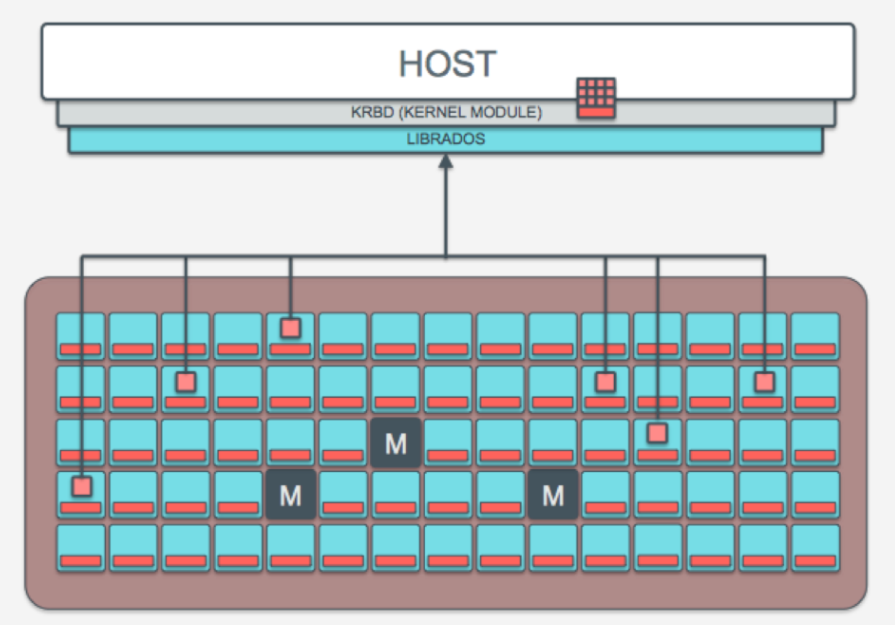
\includegraphics[width=0.7\linewidth]{rbd-native.png}
    \end{figure}
    \textbf{Machines can mount an RBD image using native linux kernel drivers} 
\end{frame}

\begin{frame}{RBD: Virtual Machines}
    \begin{itemize}
        \item \textbf{The \textit{librbd} library}
            \begin{itemize}
                \item Maps data blocks into objects for storage in the Ceph Object Store
                \item Inherit \textit{librados} capabilities such as snapshots and clones
            \end{itemize}
        \item \textbf{Virtualization containers}
            \begin{itemize}
                \item KVM or QEMU can use VM images that are stored in RADOS
                \item Virtualization containers can also use RBD block storage in OpenStack and CloudStack platforms
            \end{itemize}
        \item \textbf{Ceph based VM Images}
            \begin{itemize}
                \item Are striped across the entire cluster
                \item Allow simultaneous read access from different cluster nodes
            \end{itemize}
    \end{itemize}
\end{frame}

\begin{frame}{RBD: Virtual Machines}
    \begin{figure}[htpb]
        \centering
        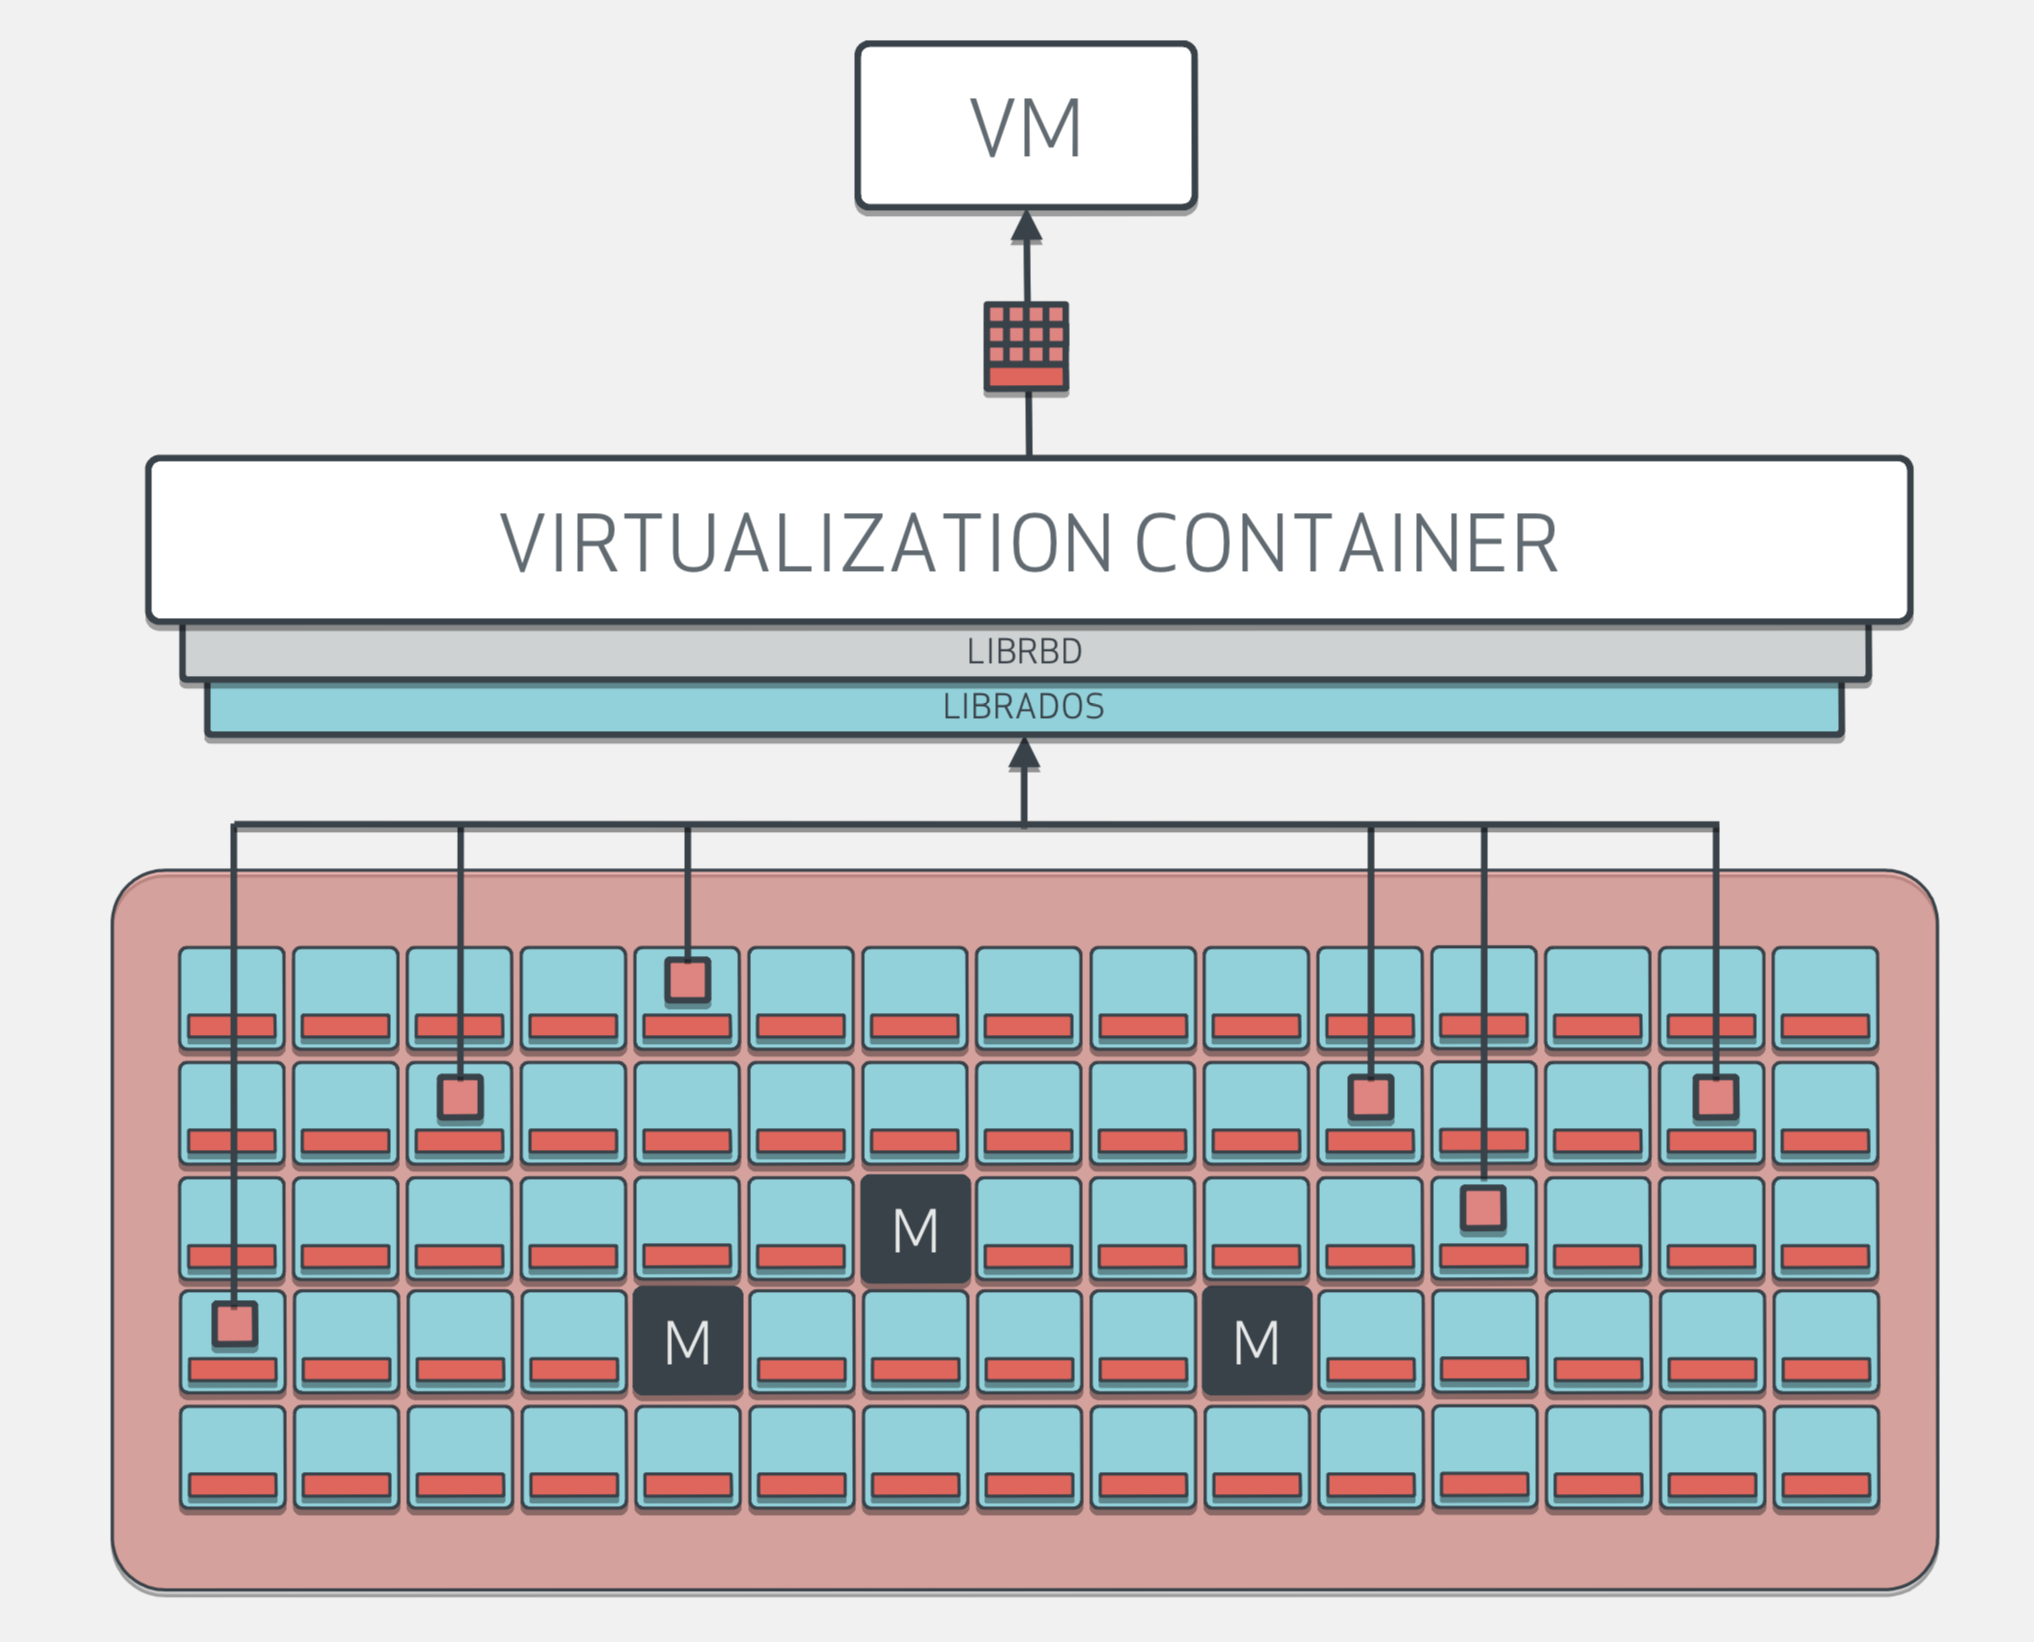
\includegraphics[width=0.7\linewidth]{rbd-vm.png}
    \end{figure}
\end{frame}

\begin{frame}[fragile]{Access RBD using librbd}
\begin{lstlisting}[language=python]
with rados.Rados(conffile='my_ceph.conf') as cluster:
    with cluster.open_ioctx('mypool') as ioctx:
        rbd_inst = rbd.RBD()
        size = 4 * 1024**3  # 4 GiB
        rbd_inst.create(ioctx, 'myimage', size)
        with rbd.Image(ioctx, 'myimage') as image:
            data = 'foo' * 200
            image.write(data, 0)
\end{lstlisting}
\end{frame}

\begin{frame}[fragile]
\begin{columns}
    \begin{column}{0.4\textwidth}
\begin{lstlisting}[language=python]
apiVersion: v1
kind: PersistentVolume
metadata:
  name: ceph-rbd-pv
spec:
  capacity:
    storage: 1Gi
  accessModes:
    - ReadWriteOnce
  rbd:
    monitors:
    - '172.31.56.105:6789'
    - '172.31.57.232:6789'
    - '172.31.58.195:6789'
    pool: rbd
    image: foo
    user: admin
    secretRef:
      name: ceph-secret
    fsType: ext4
    readOnly: false
\end{lstlisting}
    \end{column}
    \begin{column}{0.4\textwidth}
\begin{lstlisting}[language=python]
apiVersion: v1
kind: PersistentVolumeClaim
metadata:
  name: ceph-rbd-pv-claim
spec:
  accessModes:
    - ReadWriteOnce
  resources:
    requests:
      storage: 1Gi
\end{lstlisting}

\begin{lstlisting}[language=python]
apiVersion: v1
kind: Pod
metadata:
  name: ceph-rbd-pv-pod1
spec:
  containers:
  - name: rbd-rw
    image: kubernetes/pause
    volumeMounts:
    - name: ceph-rbd-vol1
      mountPath: /mnt/rbd
      readOnly: false
  volumes:
  - name: ceph-rbd-vol1
    persistentVolumeClaim:
      claimName: ceph-rbd-pv-claim
\end{lstlisting}
    \end{column}
\end{columns}
\end{frame}


\section{Ceph Filesystem}

%\subsection{System Architecture}

\begin{frame}{System Architecture}
    \begin{figure}[htpb]
        \centering
        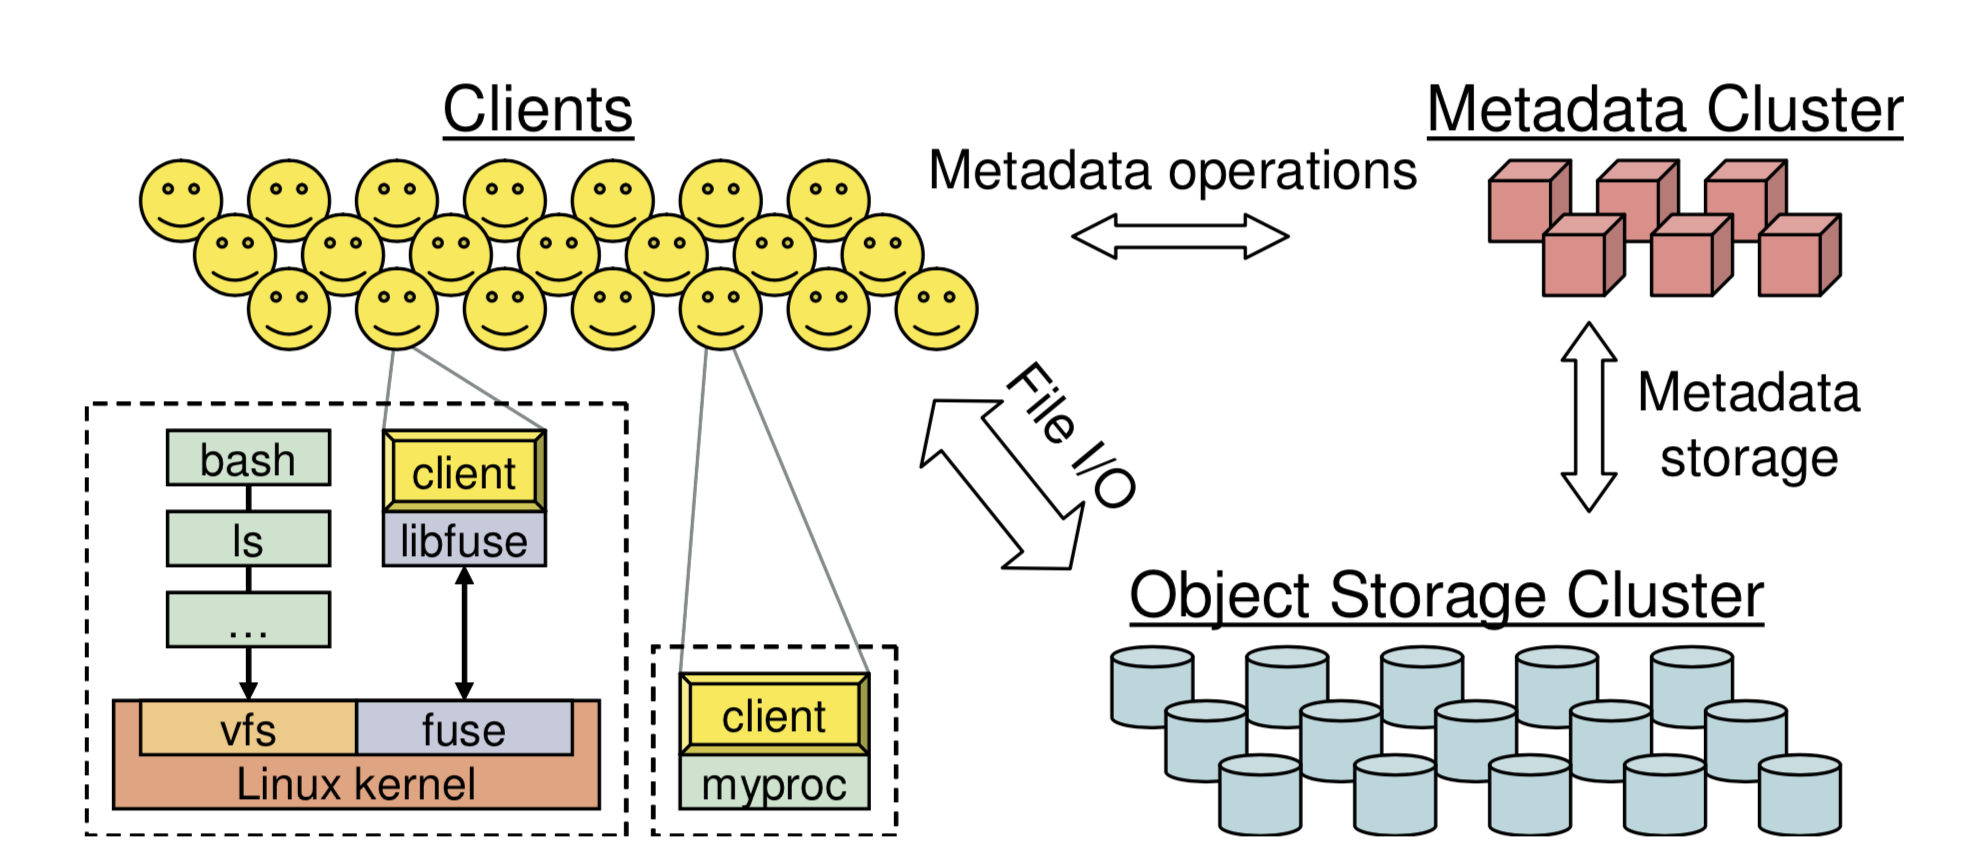
\includegraphics[width=0.8\linewidth]{cephfs-architecture.png}
    \end{figure}
\end{frame}

\begin{frame}{System Architecture}
    \begin{itemize}
        \item \textbf{Clients}
            \begin{itemize}
                \item Export a near-POSIX file system interface
            \end{itemize}
        \item \textbf{Cluster of OSDs}
            \begin{itemize}
                \item Store all data and metadata
                \item Communicate directly with clients
            \end{itemize}
        \item \textbf{Metadata Server Cluster}
            \begin{itemize}
                \item Manages the namespace (files + directories)
                \item Security, consistency and coherence
            \end{itemize}
    \end{itemize}
\end{frame}

\begin{frame}{Key Ideas}
    \begin{itemize}
        \item \textbf{Seperate data and metadata management tasks}
        \item \textbf{Dynamic partitioning of metadata data tasks inside metadata cluster}
            \begin{itemize}
                \item Avoid hot spots
            \end{itemize}
        \item \textbf{Let OSDs handle file migration and replication tasks}
    \end{itemize}
\end{frame}

%\subsection{Ceph Metadata Server}

\begin{frame}[fragile]{Create and Mount CephFS}
\begin{lstlisting}[language=python]
## creating pools
$ ceph osd pool create cephfs_data 128
$ ceph osd pool create cephfs_metadata 128
## creating a file system
$ ceph fs new cephfs cephfs_metadata cephfs_data
$ ceph fs ls
name: cephfs, metadata pool: cephfs_metadata, data pools: [cephfs_data ]
\end{lstlisting}

\begin{lstlisting}[language=python]
## there are 2 ways to mount a file system
## ceph-fuse is most of the time slower than the cephfs kernel module

## mount cephfs with the kernel driver
$ sudo mkdir /mnt/mycephfs
$ sudo mount -t ceph 192.168.0.1:6789:/ /mnt/mycephfs

## mount cephfs using fuse
$ sudo mkdir /home/username/cephfs
$ sudo ceph-fuse -m 192.168.0.1:6789 /home/username/cephfs
\end{lstlisting}
\end{frame}

\begin{frame}{MDS High Availabilty}
    \begin{itemize}
        \item MDSs can be running in two modes
            \begin{itemize}
                \item active
                \item standby
            \end{itemize}
        \item A standby MDS can become active
            \begin{itemize}
                \item If the previously active daemon goes away
            \end{itemize}
        \item Multiple active MDSs for load balancing
            \begin{itemize}
                \item Are a possibility
                \item This configuration is currently not supported/recommended
            \end{itemize}
    \end{itemize}
\end{frame}

\begin{frame}{MDS Functionality}
    \begin{itemize}
        \item The client learns about MDSs and OSDs from MON
            \begin{itemize}
                \item via MON Map, OSD Map and MDS Map
            \end{itemize}
        \item Clients talk to MDS for access to Metadata
            \begin{itemize}
                \item Permission bits, ACLs, file ownership, etc.
            \end{itemize}
        \item Clients talk to OSD for access to data
        \item MDSs themselves store all their data in OSDs
            \begin{itemize}
                \item In a separate pool called metadata
            \end{itemize}
    \end{itemize}
\end{frame}

\begin{frame}{MDS Functionality}
    \begin{figure}[htpb]
        \centering
        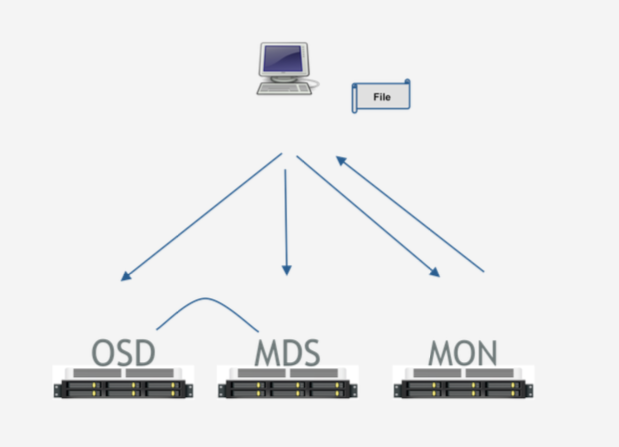
\includegraphics[width=0.8\linewidth]{cephfs-mds.png}
    \end{figure}
\end{frame}

\begin{frame}{Client Access Example}
    \begin{itemize}
        \item Client sends open request to MDS
        \item MDS returns capability, file inode, file size and stripe information
            \begin{itemize}
                \item capability specifies authorized operations on file
            \end{itemize}
        \item Client read/write directly from/to OSDs
        \item MDS manages the capability
        \item Client sends close request, relinquishes capability, provides details to MDS
    \end{itemize}
\end{frame}

%\subsection{Dynamic Tree Partitioning}

\begin{frame}{Metadata management}
    \begin{itemize}
        \item Metadata operations often make up as much as half of file system workloads...
        \item \textbf{Dynamic Subtree Partitioning}
            \begin{itemize}
                \item Lets Ceph dynamically share metadata workload among tens or hundreds of metadata servers(MDSs)
                \item Sharing is dynamic and based on current access patterns
            \end{itemize}
        \item Results in near-linear performance scaling in the number of MDSs
    \end{itemize}
\end{frame}

%\begin{frame}{Storing metadata}
%    \begin{itemize}
%        \item Most requests likely to be satisfied from MDS in-memory cache
%        \item Each MDS lodges its update operations in lazily-flushed journal
%            \begin{itemize}
%                \item Facilitates recovery
%            \end{itemize}
%        \item Directories
%            \begin{itemize}
%                \item Include i-nodes
%                \item Stored on a OSD cluster
%            \end{itemize}
%    \end{itemize}
%\end{frame}
%
%\begin{frame}{Dynamic Subtree Partitioning}
%    \begin{itemize}
%        \item Ceph uses primary copy approach to cached metadata management
%        \item Ceph adaptively distributes cached metadata across MDS nodes
%            \begin{itemize}
%                \item Each MDS measures popularity of data within a directory
%                \item Ceph migrates and/or replicates hot spots
%            \end{itemize}
%    \end{itemize}
%\end{frame}

\begin{frame}{Mapping Subdirectories to MDSs}
    \begin{figure}[htpb]
        \centering
        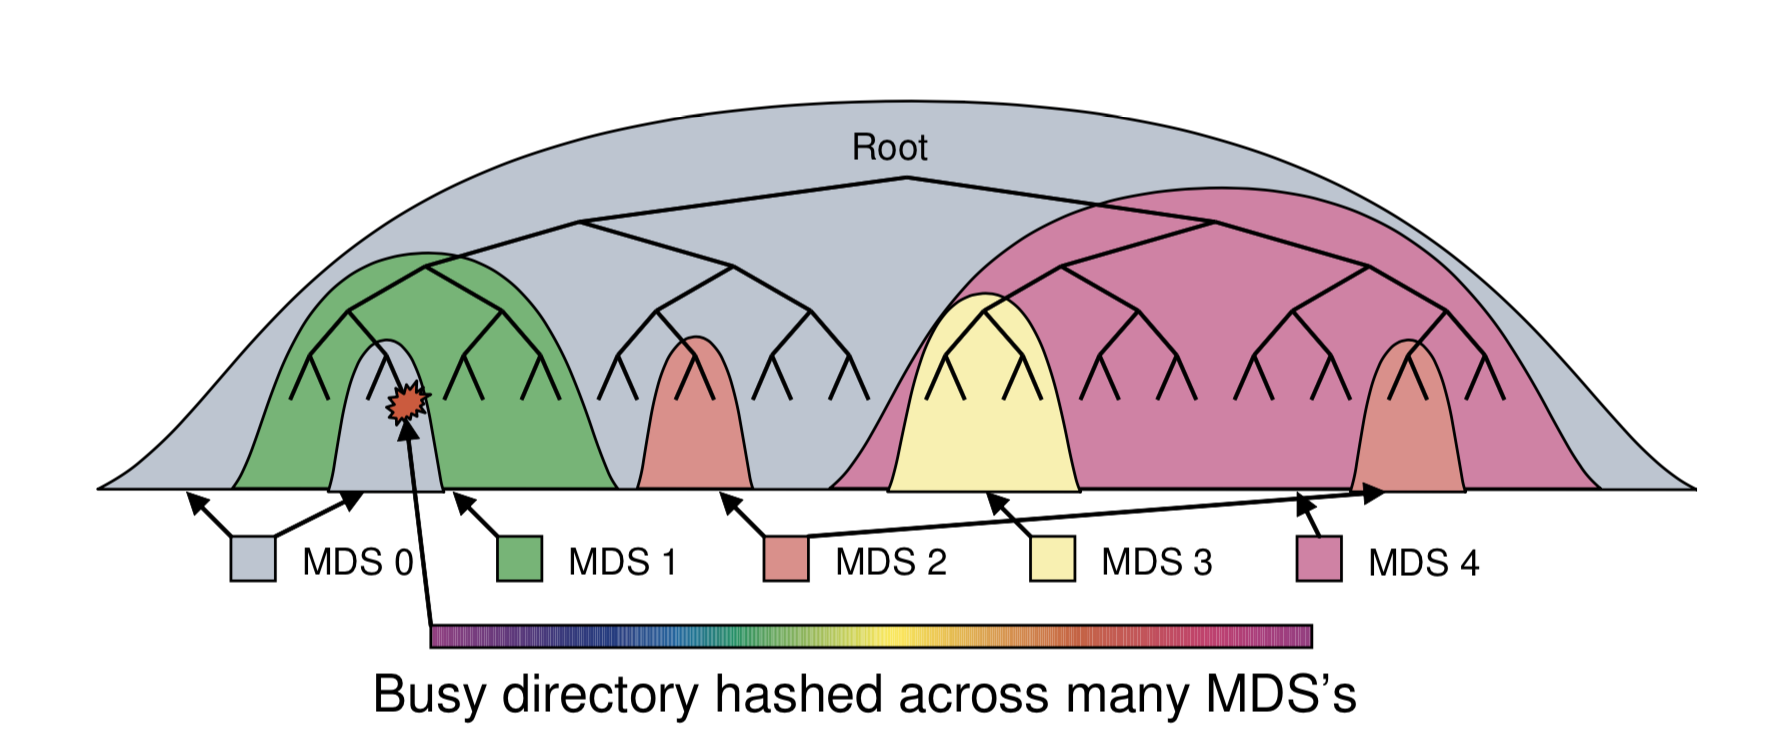
\includegraphics[width=0.8\linewidth]{cephfs-dtp.png}
    \end{figure}
\end{frame}

\begin{frame}[fragile]
\begin{columns}
    \begin{column}{0.4\textwidth}
\begin{lstlisting}[language=python]
apiVersion: v1
kind: PersistentVolume
metadata:
  name: cephfs-pv
spec:
  capacity:
    storage: 10Gi
  accessModes:
    - ReadWriteMany
  cephfs:
    monitors:
    - '172.31.56.105:6789'
    - '172.31.57.232:6789'
    - '172.31.58.195:6789'
    user: admin
    secretRef:
      name: ceph-secret
    readOnly: false
\end{lstlisting}

\begin{lstlisting}[language=python]
kind: PersistentVolumeClaim
apiVersion: v1
metadata:
  name: cephfs-pv-claim
spec:
  accessModes:
    - ReadWriteMany
  resources:
    requests:
      storage: 10Gi
\end{lstlisting}
    \end{column}
    \begin{column}{0.4\textwidth}
      
\begin{lstlisting}[language=python]
apiVersion: v1
kind: Pod
metadata:
  labels:
    test: cephfs-pvc-pod
  name: cephfs-pv-pod1
spec:
  containers:
  - name: cephfs-pv-busybox1
    image: busybox
    command: ["sleep", "60000"]
    volumeMounts:
    - mountPath: "/mnt/cephfs"
      name: cephfs-vol1
      readOnly: false
  volumes:
  - name: cephfs-vol1
    persistentVolumeClaim:
      claimName: cephfs-pv-claim
\end{lstlisting}
    \end{column}
\end{columns}
\end{frame}


\section{Conclusions}
\subsection{Conclusions}

\begin{frame}

\end{frame}



\end{document}
